\documentclass[times, utf8, diplomski]{fer}

\usepackage{booktabs}
\usepackage[hidelinks]{hyperref}
\usepackage{pdfpages}
\usepackage{float}
\usepackage{caption}
\usepackage{subcaption}
\usepackage{algorithm2e}
\usepackage{pgffor}

\SetAlgorithmName{Algoritam}{List of algorithms}{}
\SetAlgoInsideSkip{smallskip}
\SetKwInput{Input}{Ulaz}
\SetKwInput{Output}{Izlaz}
\RestyleAlgo{ruled}
\SetKwFor{ForEach}{za svaki}{radi}{kraj}
\SetKwFor{While}{dok}{radi}{kraj}

\DeclareMathOperator*{\argmax}{arg\,max}

\begin{document}

\thesisnumber{3036}
\title{Automatsko prepoznavanje registarskih tablica pomoću dubokih modela}
\author{Darijo Brčina}

% \maketitle

% Ispis stranice s napomenom o umetanju izvornika rada. Uklonite naredbu \izvornik ako želite izbaciti tu stranicu.
% \izvornik
% 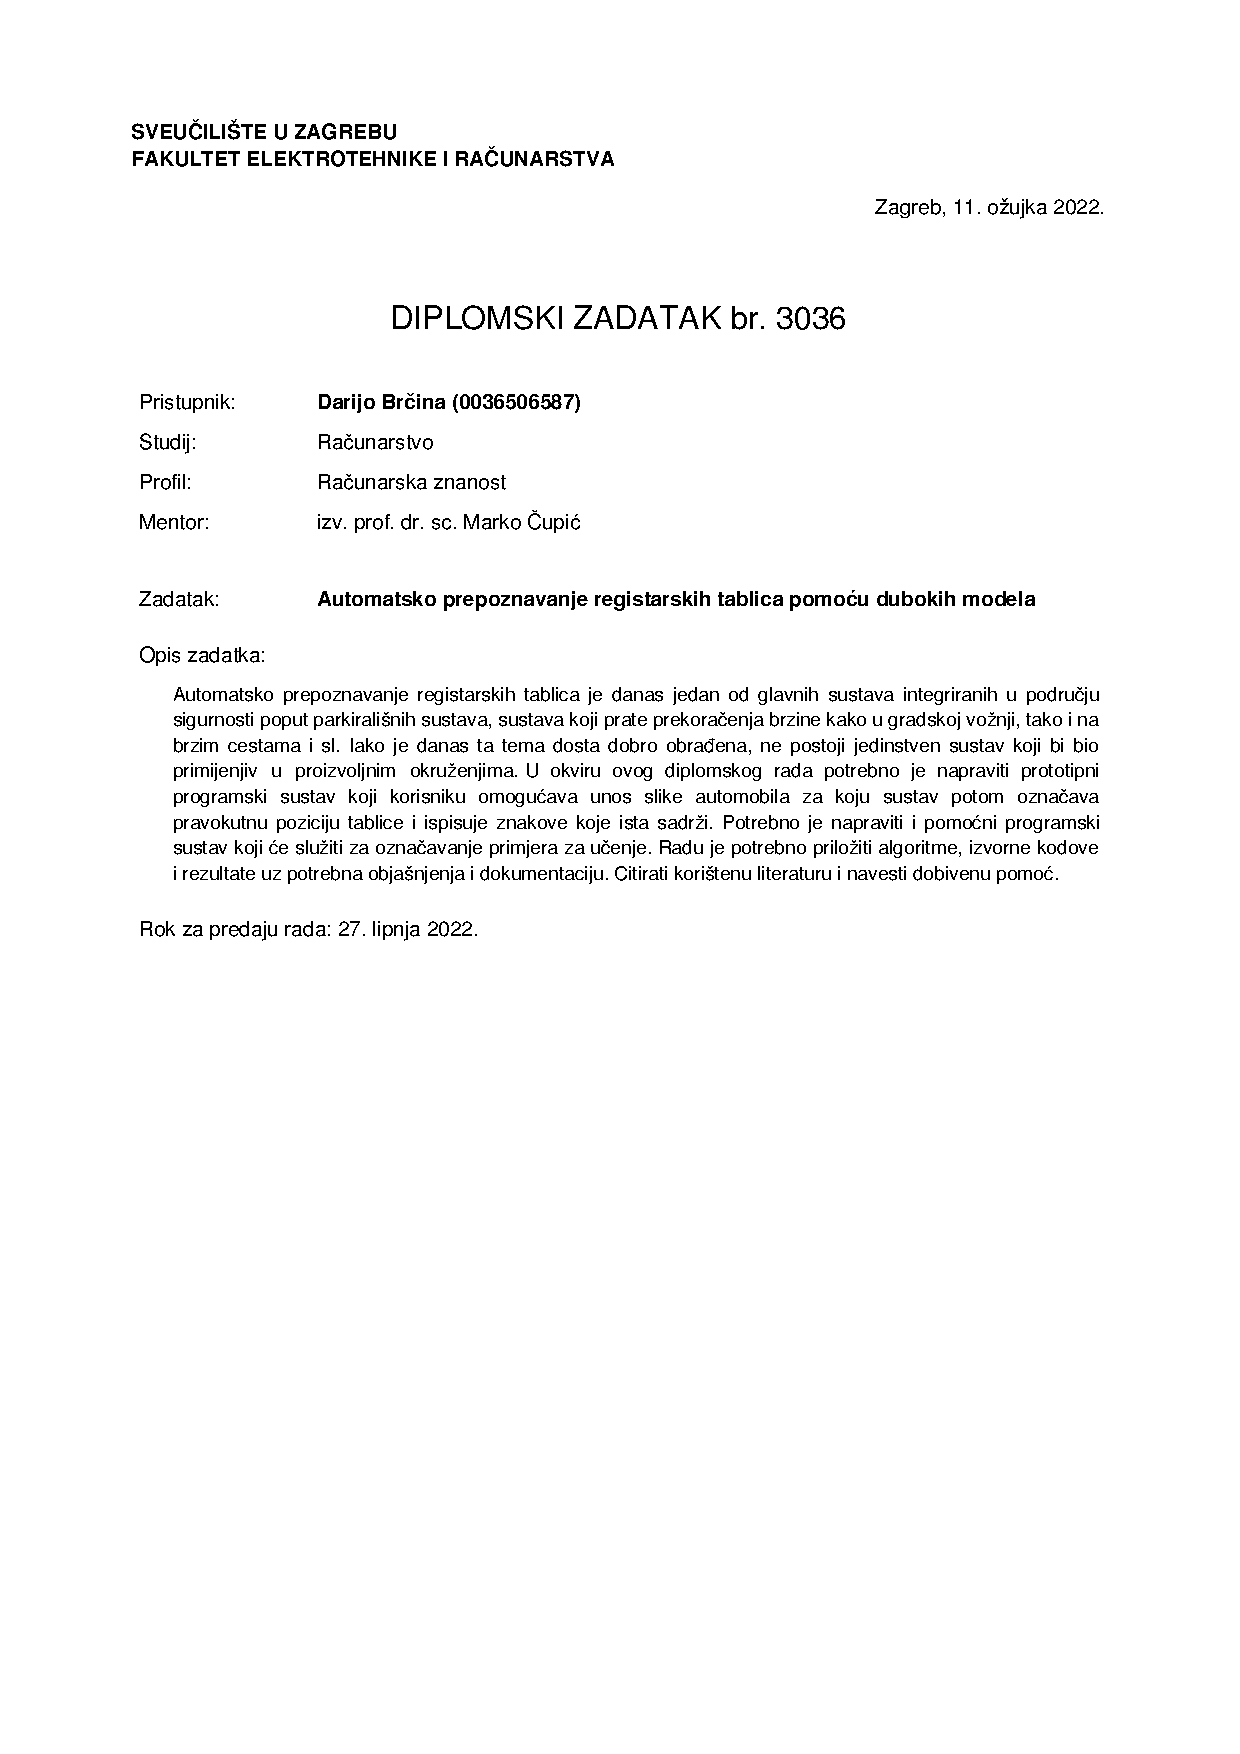
\includepdf[pages=-]{zadatak}

% Dodavanje zahvale ili prazne stranice. Ako ne želite dodati zahvalu, naredbu ostavite radi prazne stranice.
\zahvala{Zahvaljujem mentoru Marku što mi je dopustio slobodan izbor teme ovog rada i uvijek znao dati kvalitetan odgovor. Uz njegovo mentorstvo sam shvatio koliko je bitno biti samostalan, što više istraživati i pokušavati pronaći rješenje nekog problema, bez konstantnog traženja pomoći. To je odlika pravog inženjera. Jednom kada zapneš, a zapet ćeš, i iscrpiš sva moguća znanja, no i dalje ne vidiš rješenje problema, tada tražiš pomoć jer znaš da više ne znaš kamo bi krenuo, ali si samouvjeren jer si uložio svoj trud i vrijeme i nije te sram. U takvim trenucima je bitno imati osobu, mentora, koji će ti na temelju svog iskustva dati dobar odgovor. To često i nije odgovor koji u potpunosti rješava problem, iako ga je sam vjerojatno svjestan, već je odgovor koji će te pogurati u smjeru kojim trebaš ići. Jer koja je čar svega, ako dobiješ odgovor koji promptno rješava problem? Treba sjesti i doći do rješenja. Upravo to sam dobio od mentora Marka. Hvala mentore.

Zahvaljujem svom drugom mentoru, Dejanu Čakiji, koji je, iako izrazito potkovan znanjem, prije svega bio moj moralni mentor. Prepoznao je moj potencijal vrlo rano, još u doba srednje škole i shodno tomu me konstantno pratio i bodrio. Jako je bitno imati i mentora koji će te emocionalno bodriti jer to je, uz bodrenje znanjem, dobitna kombinacija. Hvala Dejane.

Zahvaljujem bratiću Stjepanu, koji je tri godine stariji i koji je također sve prolazio što sam i ja prolazio, na svoj ukazanoj pomoći i usmjeravanju kroz studij. Na početku je to neizmjerno značilo.

Zahvaljujem svim svojim prijateljima koji su cijelo vrijeme bili uz mene i uz ovaj moj put. Sve ovo bi bez vas bilo besmisleno. Prepoznat ćete se.

Na kraju, najveća zahvala ide mojoj obitelji, bratu Danijelu, tati Zoranu i mami Katici. Za mene, najvrjedniji mentori. Sve ste svjedočili, sve ste osjetili, sve (ni)ste podupirali, a sve i financirali. Sada je red na meni. Ostale riječi nisu potrebne jer je sve kristalno jasno. Volim vas, a pogotovo svoju majku.}

\tableofcontents

\chapter{Uvod}
Automatsko prepoznavanje registarskih tablica \engl{automatic license plate recognition} je danas jedan od najkorištenijih sustava u području sigurnosti i nadzora. Otvaranje rampi za ulazak na parkirališne zone i garaže, plaćanje cestarina, provjera plaćanja parkinga na javnoj površini, praćenje automobila koji prelaze ograničenja brzine, prolasci kroz crvena svjetla itd.\ su samo neki od primjena. S obzirom na to da se takvi sustavi koriste u izrazito rizičnoj domeni primjene, isti moraju biti kvalitetno implementirani i testirani.

U ovom radu dan je kratak teorijski osvrt jednostavnog sustava za prepoznavanje registarskih tablica. Uz teorijski osvrt, izrađen je jedan takav sustav čiji su rezultati obećavajući.

\bigskip

U drugom poglavlju dan je kratak pregled područja i srodnih radova. U trećem i četvrtom poglavlju dan je vrlo detaljan opis sustava za detekciju registarskih tablica i sustava za prepoznavanje registarskih tablica. U petom poglavlju prikazani su rezultati konačnog sustava i identifikacija mogućih problema. 


\chapter{Pregled područja}
Problematika teme ovog rada je već jako dobro razrađena s obzirom na jako široku i bitnu primjenu. Postoji mnoštvo različitih pristupa i tehnika od algoritama računalnog vida i obrade slika do područja strojnog i dubokog učenja. Neki od poznatijih radova u području računalnog vida pokušavaju detektirati registarske tablice pomoću Houghove transformacije \citep{hough-paper} i operatora za detekciju rubova \citep{canny-paper}, neki se služe vrlo poznatim tipovima značajki poput HOG \citep{hog-paper}, Haar \citep{haar-paper} i SIFT \citep{sift-paper} koje kombiniraju s modelima strojnog učenja, dok se ostala velika većina okreće dubokim modelima i dubokom učenju. Za detekciju objekata postoji cijela jedna serija pristupa gdje je svaki sljedeći rad nadogradnja prethodnog, a radi se o R-CNN arhitekturama koju ćemo objasniti kasnije u radu. Osnovna R-CNN arhitektura opisana je u radu \citep{rcnn-paper}, poboljšanje iste nazvano je \textit{Fast R-CNN} i opisano je u radu \citep{fast-rcnn-paper}, a konačno poboljšanje nazvano je \textit{Faster R-CNN} i opisano je u radu \citep{faster-rcnn-paper}. Kako i sama imena nalažu, radi se o očitim poboljšanjima što se tiče brzine izvođenja sustava za detekciju kao i njihovoj efikasnosti. Možda najveći obrat u području detekcije objekata su modeli koji željene objekte mogu detektirati u jednom prolazu kroz sliku \engl{single shot detectors, SSD}. Jedan od najpoznatijih modela je YOLO od \textit{you only look once} koji je opisan u radu \citep{yolo-paper}.

Što se tiče pristupa za sustave za prepoznavanje, njima se pristupa ponajviše iz perspektive obrade prirodnog jezika \engl{natural language processing, NLP} gdje povratne neuronske mreže imaju jako veliku ulogu. Jedan od revolucionarnijih radova za prepoznavanje registarskih tablica je \citep{crnn-paper} na kojem je ovaj rad i baziran. Isti povezuje razne duboke modele, no glavna riječ i dalje ostaje na povratnim neuronskim mrežama.

Studentski projekt \citep{zemris} je koristan jer implementira sustav za prepoznavanje registarskih tablica od nule.

Jako dobar pregled skoro svih mogućih pristupa za detekciju i prepoznavanje registarskih tablica iz perspektive računalnog vida i strojnog učenja nalazi se u radu \citep{survey}, dok su navedeni radovi za YOLO i R-CNN dobre odskočne daske za pristup pomoću dubokog učenja.


\chapter{Detekcija registarskih tablica}
Prvi korak sustava za prepoznavanje registarskih tablica je detekcija istih. Potrebno je ostvariti algoritam koji bi, na temelju predane slike, trebao biti u stanju izdvojiti jedan ili više potencijalnih dijelova slike koji dijele veliku sličnost s definicijom registarske tablice. Ovom problemu se može pristupiti iz nekoliko smjerova, poput korištenja algoritama za obradu slike (\textit{npr}.\ detekcija linija pomoću Houghove transformacije \citep{hough-paper}, detekcija rubova pomoću \textit{Canny} operatora \citep{canny-paper}) koji pronalaze potencijalne kosture tablica koji se daljnjom analizom filtriraju. Neke od analiza mogu biti zadovoljava li pronađeno područje određeni omjer visine i širine,  zadovoljava li određeni broj piksela i sl.

Navedeni pristupi su izrazito efikasni kada je riječ o brzini provedbe i pokazuju jako dobre rezultate kod idealnih situacija bez previše neželjenog šuma, rotacija i sl., što naravno nije realna situacija. Također, broj lažno pozitivnih \engl{false positive} područja raste kako kompleksnost slike raste (\textit{i.e}.\ prisustvo pravokutnih područja poput raznih reklama i natpisa izrazito povećava šum) te korištenje istih ne doprinosi robusnosti sustava. Navedeni problem rješava se uporabom algoritama strojnog učenja \engl{machine learning}. Za svaku registarsku tablicu se pokušava konstruirati određeni skup značajki koji će u velikoj većini slučajeva razlikovati istu od npr.\ tekstualne reklame te tako izrazito umanjiti broj lažno pozitivnih primjera. Neki od poznatijih pristupa su konstruiranje značajki pomoću histograma usmjerenih gradijenata \engl{histogram of oriented gradients} \citep{hog-paper}, poznatije kao HOG značajke te konstrukcija Haralickovih značajki \engl{Haar-like features} \citep{haar-paper}. Iako navedeni pristupi u praksi pokazuju dosta dobre rezultate, danas se ne upotrebljavaju u tolikoj mjeri zbog pojave konvolucijskih neuronskih mreža, koje su u stanju generirati puno bogatiji skup značajki. Upravo je na njima fokus ovog rada. Jednom kada se značajke izgeneriraju, prosljeđuju se nekom od modela strojnog učenja poput stroja potpornih vektora \engl{support vector machine, SVM}, \textit{AdaBoost} od \textit{Adaptive Boosting} ili neke od varijacija unaprijedne potpuno povezane neuronske mreže kako bi isti efikasno mogao naučiti klasificirati pripada li dani uzorak skupu registarskih tablica ili ne pripada. Sve navedeno je zapravo vrlo jednostavno za realizirati jednom kada imamo potencijalna područja interesa \engl{regions of interest}. No, upravo je pronalazak tih područja jedan od glavnih problema s kojim se svi algoritmi detekcije objekata suočavaju. O tome ćemo nešto više reći u sekciji Pronalaženje područja interesa.

\bigskip

Rezimirajmo poglavlje i prikažimo hodogram izgradnje jednog sustava za detekciju registarskih tablica. Prvi korak je prikupljanje "dovoljnog" broja slikovnih primjera koji će služiti za učenje modela\footnote{Riječ "dovoljno" je namjerno stavljena u navodnike jer u području strojnog učenja zapravo ona i ne postoji kao takva. Broj primjera za učenje nikada ne može biti prevelik i često je u praksi relativno malen, što je za izgradnju jednog prototipnog sustava sasvim dovoljno.}. Zatim je slike potrebno malo obraditi i izabrati algoritam koji pronalazi područja interesa. Nakon pronalaska područja interesa, potrebno je izabrati algoritam za izlučivanje značajki \engl{feature extraction} pomoću kojeg će se sirovi podaci transformirati u podatke koje će model moći obraditi. Nakon generiranja značajki dolazi korak u kojem se model uči na primjerima za učenje, tzv.\ faza učenja modela. Jednom naučeni model se zatim može koristiti za klasifikaciju pripada li trenutno područje interesa skupu registarskih tablica ili ne pripada, tzv.\ faza iskorištavanja modela.

U nastavku ćemo detaljnije proći kroz neke od navedenih koraka.

\section{Poboljšanje kontrasta}
Podaci koji nastaju u realnim situacijama su sve samo ne idealni kao oni na koje smo navikli kada istražujemo u kontroliranom okruženju. Jedan od čestih problema s kojim se susrećemo u obradi slike je jako loš kontrast. Naime, slike mogu biti tamne, mogu biti svijetle, na dijelovima mogu biti pod sjenom a na drugim dijelovima pod svjetlom i sl. Na slici \ref{fig:ce_originals} su prikazana četiri primjera iz baze slika koji potkrepljuju navedeno.

Kako bi sustav za detekciju i prepoznavanje registarskih tablica bio robusniji, potrebno je napraviti postupak koji se u literaturi naziva poboljšanje kontrasta \engl{contrast enhancement} \citep{szeliski}. Postoji veliki broj postupaka kojima se to može izvesti. Glavna podjela je na algoritme koji izvode transformacije u prostornoj \engl{spatial} domeni i na algoritme koji izvode transformacije u frekvencijskoj \engl{frequency} domeni. Jedna od glavnih primjena u frekvencijskoj domeni su Fourierove transformacije i to nije razmatrano u ovom radu, već je glavni fokus stavljen na transformacije u prostornoj domeni.

Hodogram za poboljšanje kontrasta je sljedeći: prvo je nad ulaznom slikom\footnote{Promatramo 8-bitne slike, što znači da su pikseli zapisani vrijednostima u rasponu $[0,255]$.} provedena konverzija iz prostora boja RGB u prostor boja YCrCb, zatim je nad Y komponentom proveden algoritam izjednačavanja histograma nakon čega je nad istom komponentom proveden Gaussov filter radi filtriranja dobivenog šuma iz prethodnog koraka. Na kraju je provedena konverzija boja u suprotnom smjeru. Dakle, iz prostora boja YCrCb u prostor boja RGB kako bi se konačna slika mogla prikazati. Zadnji korak je potreban zbog algoritma za pronalaženje područja interesa koji se obrađuje u sljedećoj sekciji. Spomenimo još da se primjeri za učenje nalaze u prostoru boja nijansi sive \engl{grayscale} zbog manjeg memorijskog utiska i bržeg izvođenja, ali o tome više kasnije.

Iako postoji mnoštvo načina za poboljšanje kontrasta, možda čak i efikasnijih, u ovom radu je navedeno rezultiralo zadovoljavajućim rezultatima. U nastavku su dani detaljniji opisi navedenih koraka.

\bigskip

\begin{figure}[H]
     \centering
     \begin{subfigure}[b]{0.4\textwidth}
         \centering
         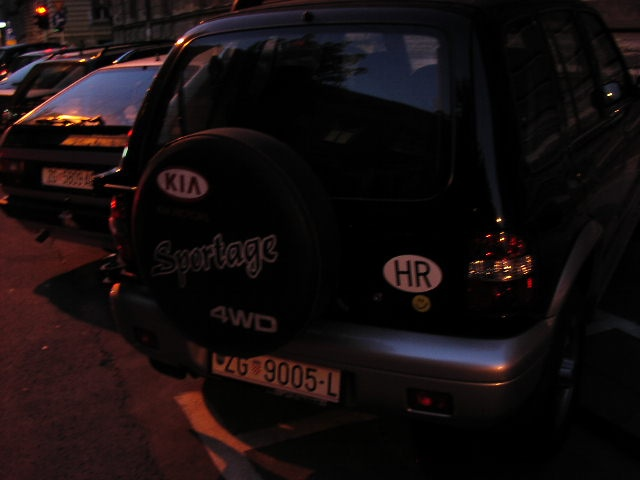
\includegraphics[width=\textwidth]{figures/ce_examples/1/original.jpg}
         \caption{Tamniji primjer}
     \end{subfigure}
     \hspace{1cm}
     \begin{subfigure}[b]{0.4\textwidth}
         \centering
         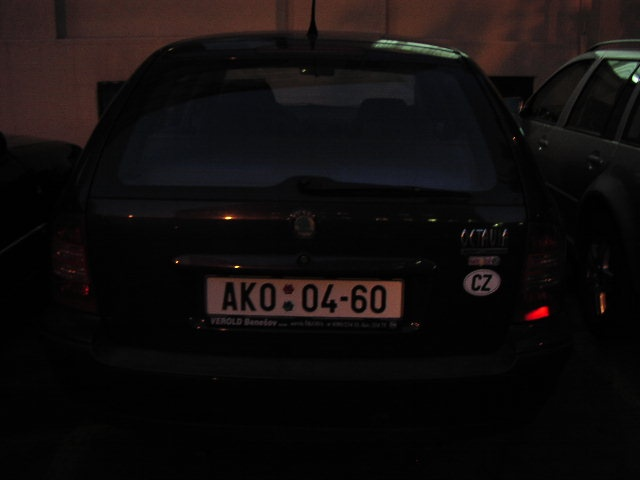
\includegraphics[width=\textwidth]{figures/ce_examples/2/original.jpg}
         \caption{Tamniji primjer uz jači kontrast}
     \end{subfigure}\\[0.5cm]
     \begin{subfigure}[b]{0.4\textwidth}
         \centering
         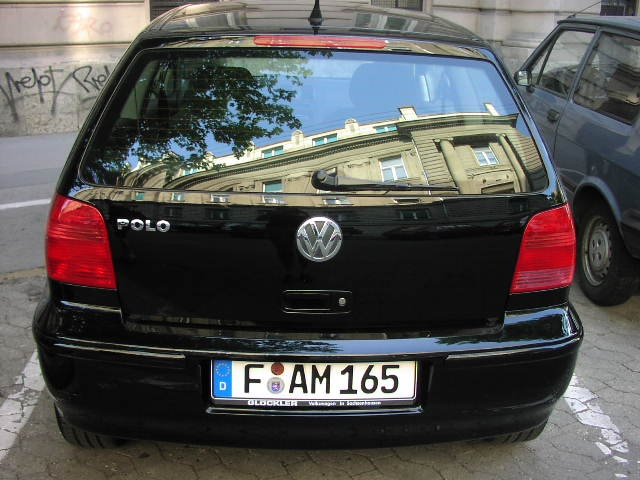
\includegraphics[width=\textwidth]{figures/ce_examples/3/original.jpg}
         \caption{Svjetliji primjer}
     \end{subfigure}
     \hspace{1cm}
     \begin{subfigure}[b]{0.4\textwidth}
         \centering
         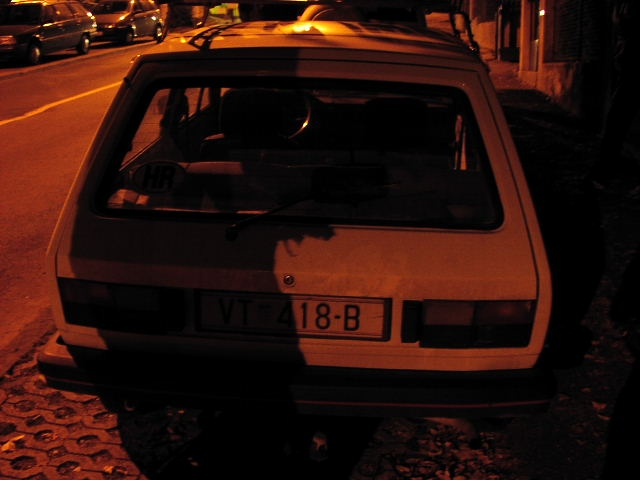
\includegraphics[width=\textwidth]{figures/ce_examples/4/original.jpg}
         \caption{Primjer sa sjenom}
     \end{subfigure}
        \caption{Primjeri originalnih slika iz baze}
        \label{fig:ce_originals}
\end{figure}

\subsection{Konverzija RGB u YCrCb}
Prostor boja YCrCb je izabran zbog svoje jednostavnosti i zbog široke rasprostranjenosti u kodiranju i dekodiranju slika i videosekvenci. Y predstavlja luminantnu \engl{luminance} komponentu, dok Cr i Cb predstavljaju krominantne \engl{chrominance} komponente razlike za crvenu i plavu boju. YCrCb je pogodan prostor boja jer se luminancija odvaja od boja, što ljudskom oku izrazito odgovara zbog puno veće osjetljivosti na luminanciju nego na boje. Na slici \ref{fig:ce_ycrcb} prikazani su primjeri konverzija prostora boja ranijih primjera sa slike \ref{fig:ce_originals}. YCrCb se koristi u JPEG kompresiji i definiran je na sljedeći način\footnote{https://docs.opencv.org/4.x/de/d25/imgproc\_color\_conversions.html}:

\begin{equation}
    Y \leftarrow 0.299 \cdot R + 0.587 \cdot G + 0.114 \cdot B,
\end{equation}
\begin{equation}
    Cr \leftarrow (R - Y) \cdot 0.713 + 128,
\end{equation}
\begin{equation}
    Cb \leftarrow (B - Y) \cdot 0.564 + 128,
\end{equation}
\begin{equation}
    R \leftarrow Y + 1.403 \cdot (Cr - 128),
\end{equation}
\begin{equation}
    G \leftarrow Y - 0.714 \cdot (Cr - 128) - 0.344 \cdot (Cb - 128),
\end{equation}
\begin{equation}
    B \leftarrow Y + 1.773 \cdot (Cb - 128).
\end{equation}

\bigskip

\begin{figure}[H]
     \centering
     \begin{subfigure}[b]{0.4\textwidth}
         \centering
         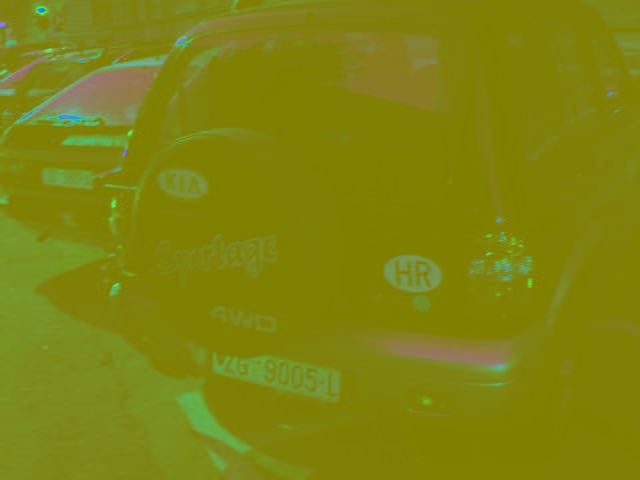
\includegraphics[width=\textwidth]{figures/ce_examples/1/ycrcb.jpg}
         \caption{Tamniji primjer}
     \end{subfigure}
     \hspace{1cm}
     \begin{subfigure}[b]{0.4\textwidth}
         \centering
         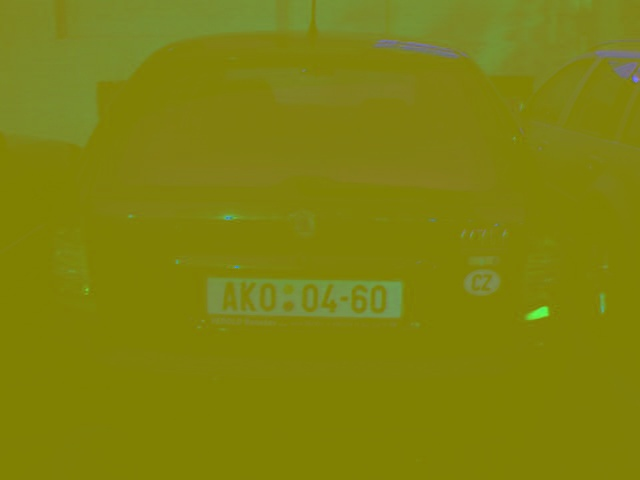
\includegraphics[width=\textwidth]{figures/ce_examples/2/ycrcb.jpg}
         \caption{Tamniji primjer uz jači kontrast}
     \end{subfigure}\\[0.5cm]
     \begin{subfigure}[b]{0.4\textwidth}
         \centering
         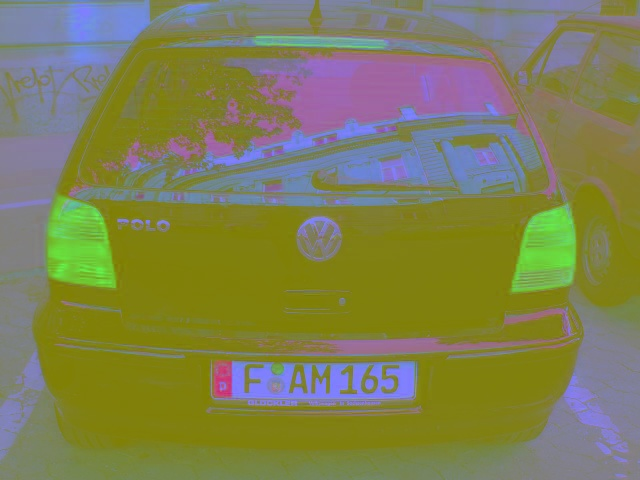
\includegraphics[width=\textwidth]{figures/ce_examples/3/ycrcb.jpg}
         \caption{Svjetliji primjer}
     \end{subfigure}
     \hspace{1cm}
     \begin{subfigure}[b]{0.4\textwidth}
         \centering
         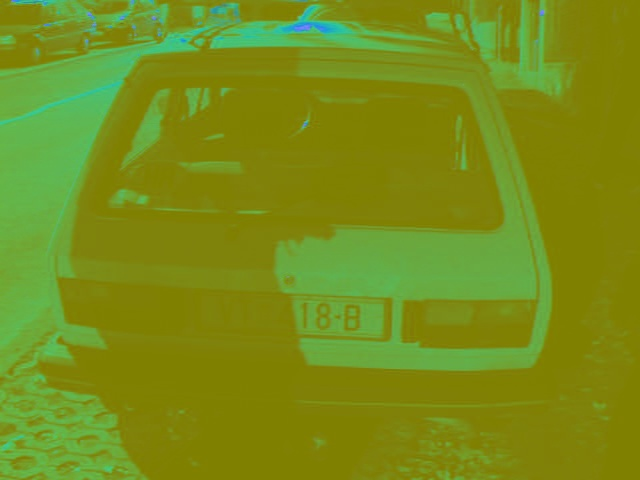
\includegraphics[width=\textwidth]{figures/ce_examples/4/ycrcb.jpg}
         \caption{Primjer sa sjenom}
     \end{subfigure}
        \caption{Primjeri konverzija ranijih slika}
        \label{fig:ce_ycrcb}
\end{figure}


\subsection{Izjednačavanje histograma}
Izjednačavanje histograma\footnote{Histogram je ništa drugo nego graf koji prikazuje koliko je svih 256 vrijednosti piksela sadržano na slici.} \engl{histogram equalization} je jedna od vrlo efikasnih tehnika kojom se poboljšava kontrast slike. Ideja je da se određeni slikovni kanali vrijednosno prošire na cijeli spektar od 256 vrijednosti piksela kako bi tamnije slike bile svjetlije te kako bi svjetlije slike bile tamnije. Da bi to bilo izvedivo, potrebno je definirati određenu funkciju koja će mapirati intenzitete piksela na takav način da rezultirajući histogram bude relativno ravan \engl{flat}, odnosno da se gotovo svaka vrijednost od mogućih 256 pridruži nekom od piksela.

U \citep{szeliski} se navedeno definira na sljedeći način: neka je $N$ broj piksela neke slike, $I$ intenzitet piksela, $h(I)$ distribucija intenziteta piksela neke slike, dakle radi se o histogramu, i $f(I)$ funkcija koja mapira intenzitete piksela. Funkcija $f(I)$ je definirana kao integral\footnote{S obzirom na to da se radi s diskretnim vrijednostima, integral je zapravo sumacija.} od distribucije intenziteta piksela $h(I)$:

\begin{equation}
    f(I) = \frac{1}{N}\sum_{i=0}^{I}h(i) = f(I-1) + \frac{1}{N}h(I).
\end{equation}

\bigskip

S obzirom na to da se radi o 8-bitnim slikama, $f(I)$ je potrebno još skalirati na interval $[0,255]$. Jednom kada imamo navedenu funkciju mapiranja, dalje je lako provesti postupak izjednačavanja histograma. Jednostavno za svaki piksel originalne slike izračunamo novu vrijednost intenziteta koju će taj piksel primiti. Na slikama \ref{fig:ce_hist_original} i \ref{fig:ce_hist_eq} se nalaze (izjednačeni) histogrami komponente Y prijašnjih slika. Na slici \ref{fig:ce_eq} se nalazi primjena izjednačenih histograma komponente Y na prijašnje slike. Dosta jasno se i po grafovima i po krajnjim rezultatima vidi da je utjecaj izjednačavanja histograma kod tamnijih slika izrazito veći nego kod svjetlijih slika.

Možda se pitate zašto je samo jedna komponenta prikazana te zašto se uopće radi s komponentom Y, a ne s ostalima. Kao što je navedeno ranije, oko je puno manje osjetljivije na boje nego na luminanciju, stoga je veći fokus dan na svjetlinu pa shodno tomu nema ni potrebe provoditi izjednačavanje histograma nad krominantnim komponentama.

\begin{figure}[H]
     \centering
     \begin{subfigure}[b]{0.4\textwidth}
         \centering
         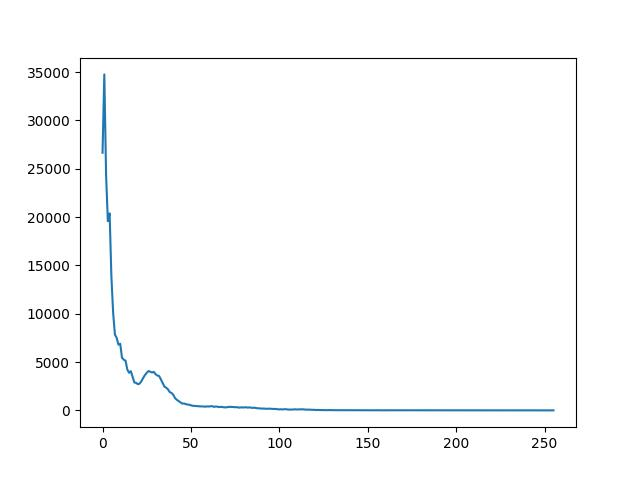
\includegraphics[width=\textwidth]{figures/ce_examples/1/hist_original.jpg}
         \caption{Tamniji primjer}
     \end{subfigure}
     \begin{subfigure}[b]{0.4\textwidth}
         \centering
         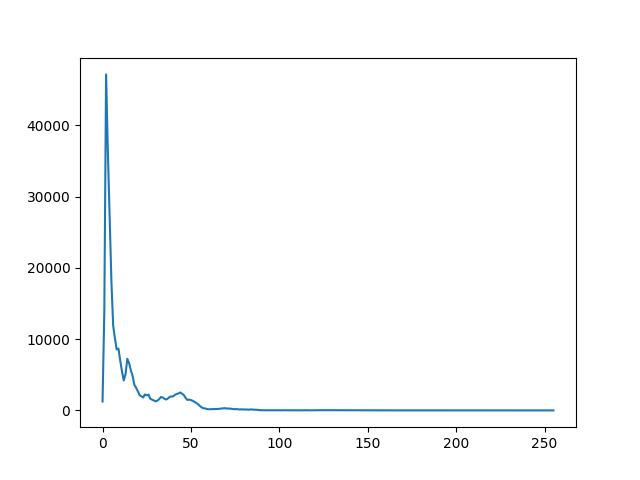
\includegraphics[width=\textwidth]{figures/ce_examples/2/hist_original.jpg}
         \caption{Tamniji primjer uz jači kontrast}
     \end{subfigure}
     \begin{subfigure}[b]{0.4\textwidth}
         \centering
         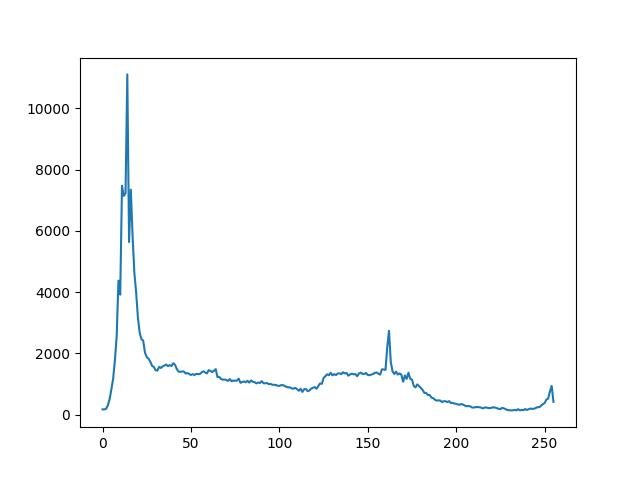
\includegraphics[width=\textwidth]{figures/ce_examples/3/hist_original.jpg}
         \caption{Svjetliji primjer}
     \end{subfigure}
     \begin{subfigure}[b]{0.4\textwidth}
         \centering
         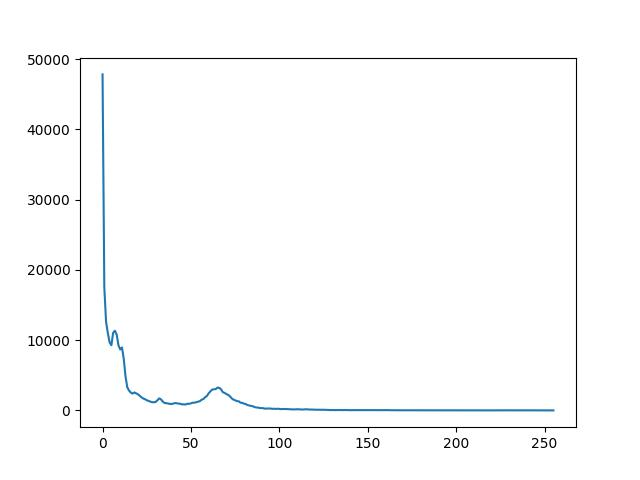
\includegraphics[width=\textwidth]{figures/ce_examples/4/hist_original.jpg}
         \caption{Primjer sa sjenom}
     \end{subfigure}
        \caption{Histogrami komponente Y}
        \label{fig:ce_hist_original}
\end{figure}

\begin{figure}[H]
     \centering
     \begin{subfigure}[b]{0.4\textwidth}
         \centering
         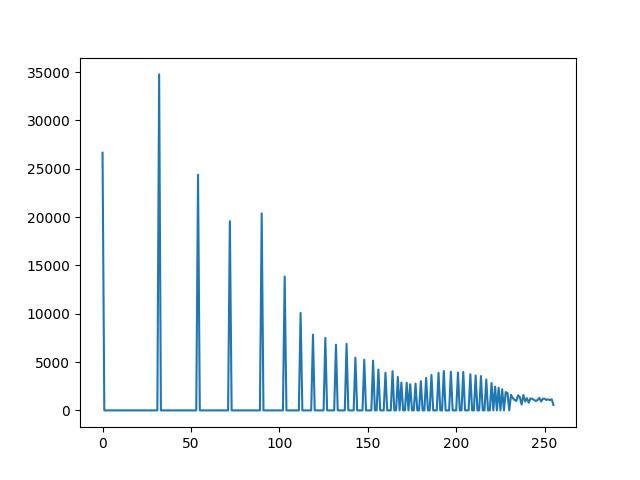
\includegraphics[width=\textwidth]{figures/ce_examples/1/hist_eq.jpg}
         \caption{Tamniji primjer}
     \end{subfigure}
     \begin{subfigure}[b]{0.4\textwidth}
         \centering
         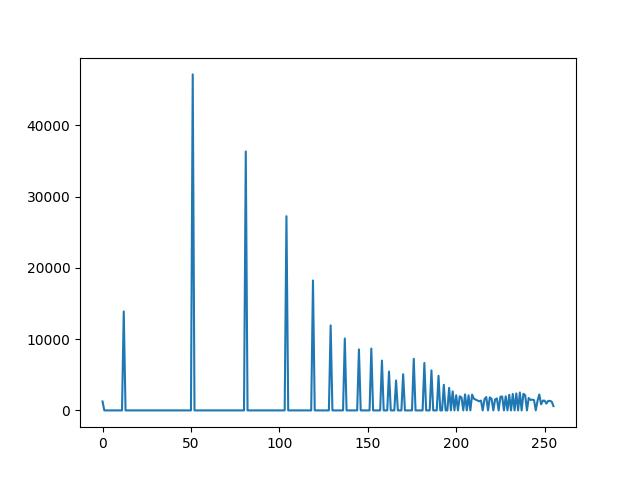
\includegraphics[width=\textwidth]{figures/ce_examples/2/hist_eq.jpg}
         \caption{Tamniji primjer uz jači kontrast}
     \end{subfigure}
     \begin{subfigure}[b]{0.4\textwidth}
         \centering
         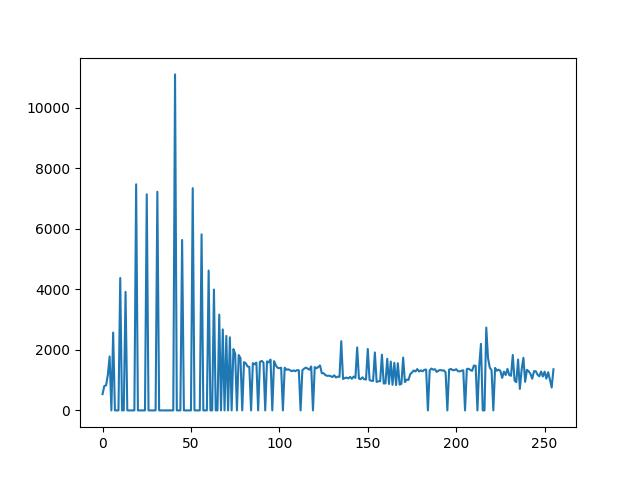
\includegraphics[width=\textwidth]{figures/ce_examples/3/hist_eq.jpg}
         \caption{Svjetliji primjer}
     \end{subfigure}
     \begin{subfigure}[b]{0.4\textwidth}
         \centering
         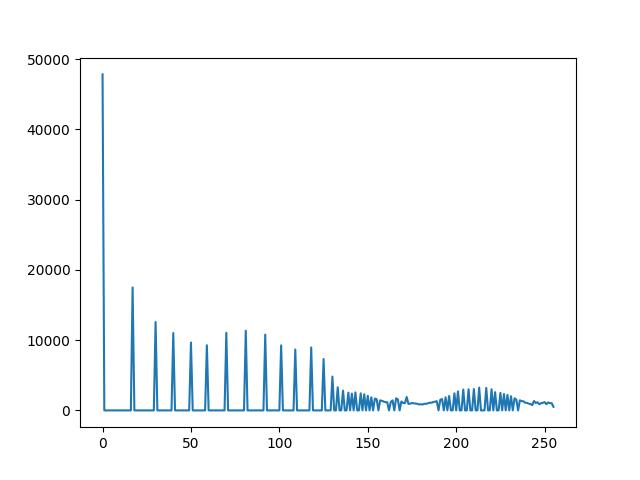
\includegraphics[width=\textwidth]{figures/ce_examples/4/hist_eq.jpg}
         \caption{Primjer sa sjenom}
     \end{subfigure}
        \caption{Izjednačeni histogrami komponente Y}
        \label{fig:ce_hist_eq}
\end{figure}

\begin{figure}[H]
     \centering
     \begin{subfigure}[b]{0.4\textwidth}
         \centering
         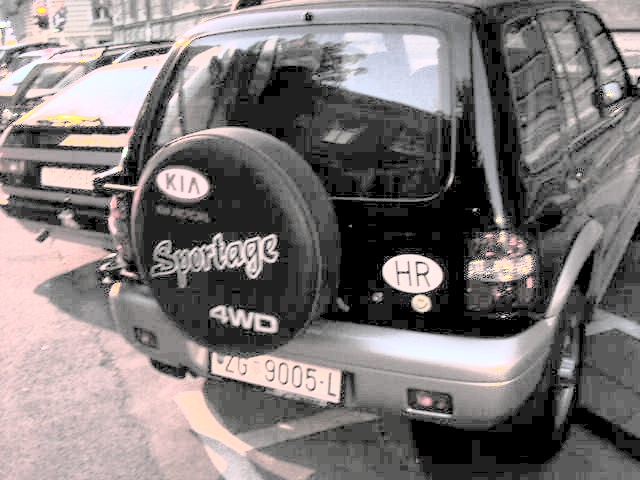
\includegraphics[width=\textwidth]{figures/ce_examples/1/eq.jpg}
         \caption{Tamniji primjer}
     \end{subfigure}
     \hspace{1cm}
     \begin{subfigure}[b]{0.4\textwidth}
         \centering
         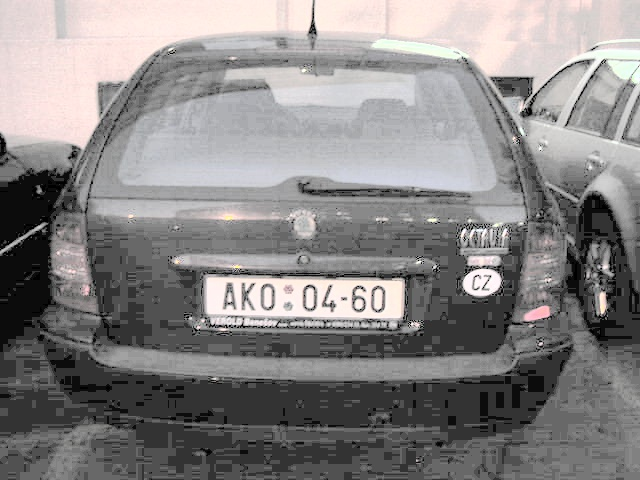
\includegraphics[width=\textwidth]{figures/ce_examples/2/eq.jpg}
         \caption{Tamniji primjer uz jači kontrast}
         \label{fig:ce_eq:sum}
     \end{subfigure}\\[0.5cm]
     \begin{subfigure}[b]{0.4\textwidth}
         \centering
         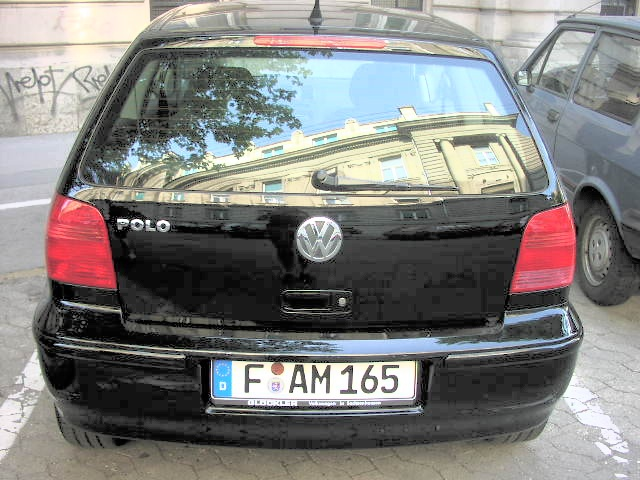
\includegraphics[width=\textwidth]{figures/ce_examples/3/eq.jpg}
         \caption{Svjetliji primjer}
     \end{subfigure}
     \hspace{1cm}
     \begin{subfigure}[b]{0.4\textwidth}
         \centering
         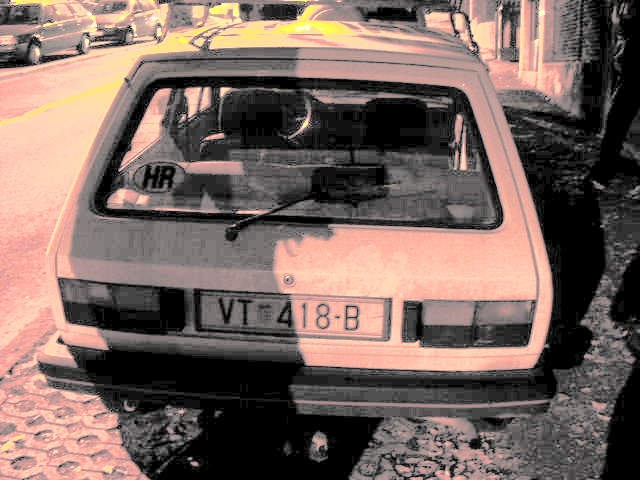
\includegraphics[width=\textwidth]{figures/ce_examples/4/eq.jpg}
         \caption{Primjer sa sjenom}
     \end{subfigure}
        \caption{Primjena izjednačenih histograma nad komponentom Y}
        \label{fig:ce_eq}
\end{figure}

Glavna mana ovakvog pristupa je uzimanje globalnog konteksta u samoj provedbi. Kao što i sam algoritam nalaže, nad svim pikselima slike se pristupa na identičan način, pa tako dijelovi koji su izrazito tamni generiraju jako puno šuma koji otežava daljnju analizu, Navedeno je dobro prikazano na slici \ref{fig:ce_eq:sum}. Šum se donekle može smanjiti primjenom raznih filtera s kojim ćemo se upoznati kasnije, ali i dalje to nije dovoljno dobro. Kako bi se navedeni problem riješio, uvodi se mala modifikacija algoritma koja provodi gotovo pa sve isto kao i prva verzija algoritma, jedino što se ta provedba vrši pomoću klizećih prozora fiksne veličine kako bi se u obzir uzelo i susjedstvo. Ova tehnika se onda naziva prilagođeno izjednačavanje histograma \engl{adaptive histogram equalization, AHE} i u ovom radu je promatrana verzija istog koja je ograničena kontrastom i naziva se prilagođeno izjednačavanje histograma ograničeno kontrastom \engl{contrast limited adaptive histogram equalization, CLAHE}.

\subsubsection{Algoritam CLAHE}
Algoritam AHE često zna pretjerano pojačati kontrast u područjima slike koji su relativno konstantni te time istovremeno i uvoditi neželjeni šum. Algoritam CLAHE koristi malu modifikaciju u kojoj vrijednosti histograma nakon neke predefinirane vrijednosti jednostavno odreže i ravnomjerno distribuira na ostale intenzitete. Mogući ishod navedenog je da neki od intenziteta opet pređu predefiniranu vrijednost, ali to je prihvatljivo jer se događa rijetko, a kada se i dogodi, ne primijeti se. Na slici \ref{fig:clahe} je navedeni postupak prikazan.

Izračun histograma i djelovanje funkcije mapiranja intenziteta piksela kroz svaki klizeći prozor i na sve piksele unutar njega je izrazito računski skupo. Kako bi se to pametnije riješilo, za sve piksele koji nisu centralni pikseli trenutnog prozora se izračunava bilinearna interpolacija \engl{bilinear interpolation} na temelju susjednih prozora. Navedeno izlazi iz okvira ovoga rada, a detalji se mogu pronaći u \citep{wiki:clahe} i \citep{szeliski}.

\bigskip

\begin{figure}[H]
    \centering
    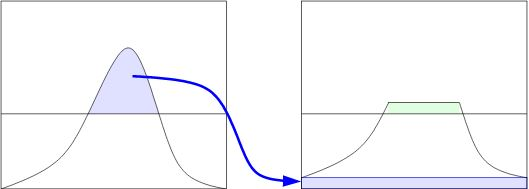
\includegraphics[scale=0.8]{figures/ce_examples/clahe.jpg}
    \caption[Caption for LOF]{Djelovanje algoritma CLAHE\footnotemark}
    \label{fig:clahe}
\end{figure}
\footnotetext{https://en.wikipedia.org/wiki/Adaptive\_histogram\_equalization}

\bigskip

Na slici \ref{fig:ce_hist_clahe} se nalaze histogrami komponente Y nakon provedbe algoritma CLAHE\footnote{Predefinirana vrijednost je 5 i veličina susjedstva je $8 \times 8$.}. Kao što se može vidjeti, histogrami su relativno slični originalnima sa slike \ref{fig:ce_hist_original}. Glavna razlika je u tome što histogrami nakon provedbe algoritma CLAHE imaju fine i zaobljene raspodijele intenziteta oko određenih vrhova. Može se reći da se histogram lijepo "razmazao" u tim dijelovima.

Na slici \ref{fig:ce_clahe} se nalaze slike nakon provedbe algoritma CLAHE nad Y komponentom. Sada se tamnije slike već puno lakše mogu raspoznati. Ovakav pristup je korišten u konačnom sustavu za detekciju i raspoznavanje registarskih tablica.

Iako se na navedenim slikama ne vidi toliko prisustvo šuma kao kod običnog algoritma izjednačavanja histograma, on je i dalje prisutan. Npr.\ na slici \ref{fig:ce_clahe_svijetli} su uzorci koji se nalaze na odrazu stražnjeg stakla izrazito potencirani ili na slici \ref{fig:ce_clahe_sjena} se po samom vozilu umjetno stvorila "prljavština" iako je taj primjer slike gotovo i nemoguće bolje obraditi zbog prisustva sjene i ulične rasvjete. U nastavku ćemo dati i potencijalno rješenje, odnosno način kojim ćemo navedene šumove barem donekle umanjiti.

\begin{figure}[H]
     \centering
     \begin{subfigure}[b]{0.4\textwidth}
         \centering
         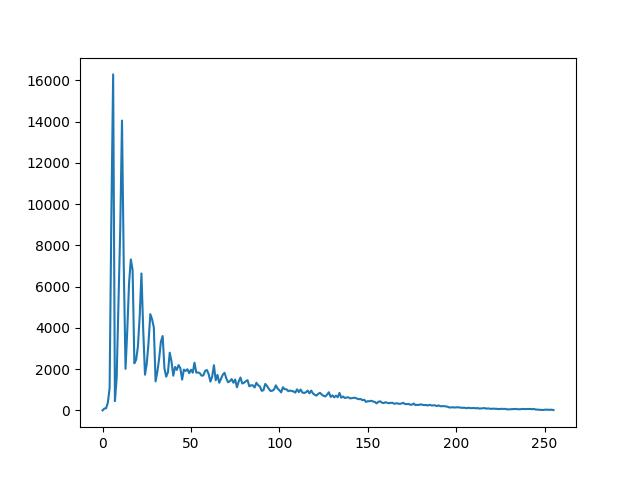
\includegraphics[width=\textwidth]{figures/ce_examples/1/hist_clahe.jpg}
         \caption{Tamniji primjer}
     \end{subfigure}
     \begin{subfigure}[b]{0.4\textwidth}
         \centering
         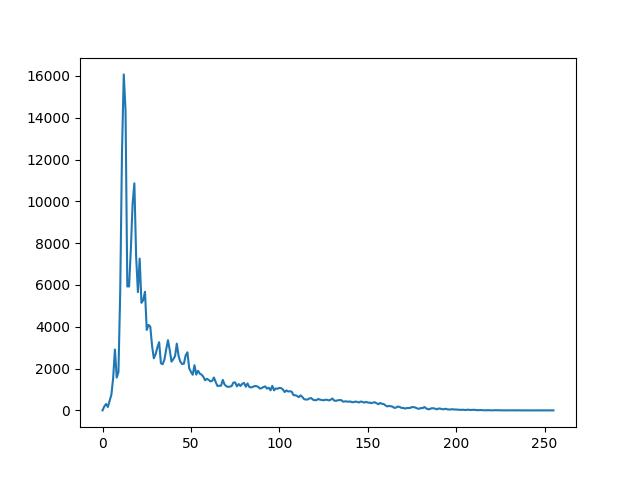
\includegraphics[width=\textwidth]{figures/ce_examples/2/hist_clahe.jpg}
         \caption{Tamniji primjer uz jači kontrast}
     \end{subfigure}
     \begin{subfigure}[b]{0.4\textwidth}
         \centering
         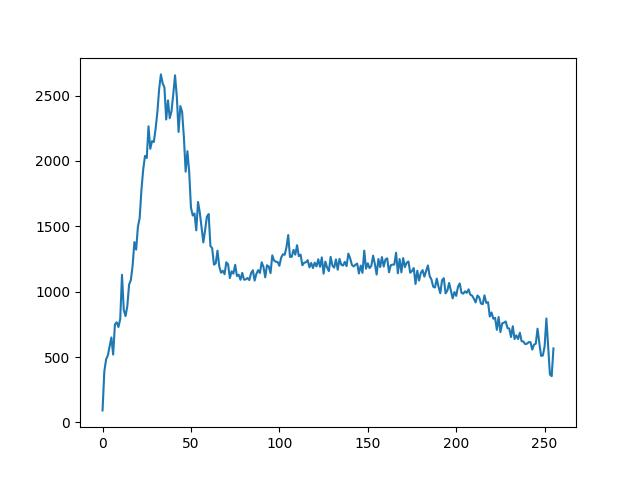
\includegraphics[width=\textwidth]{figures/ce_examples/3/hist_clahe.jpg}
         \caption{Svjetliji primjer}
     \end{subfigure}
     \begin{subfigure}[b]{0.4\textwidth}
         \centering
         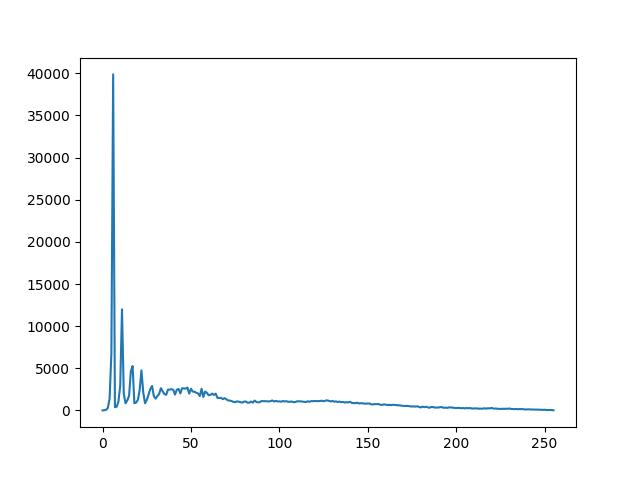
\includegraphics[width=\textwidth]{figures/ce_examples/4/hist_clahe.jpg}
         \caption{Primjer sa sjenom}
     \end{subfigure}
        \caption{Izjednačeni histogrami komponente Y algoritmom CLAHE}
        \label{fig:ce_hist_clahe}
\end{figure}

\begin{figure}[H]
     \centering
     \begin{subfigure}[b]{0.4\textwidth}
         \centering
         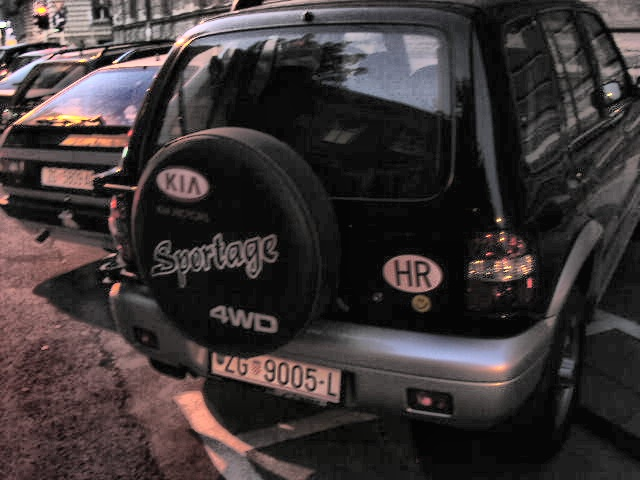
\includegraphics[width=\textwidth]{figures/ce_examples/1/clahe.jpg}
         \caption{Tamniji primjer}
     \end{subfigure}
     \hspace{1cm}
     \begin{subfigure}[b]{0.4\textwidth}
         \centering
         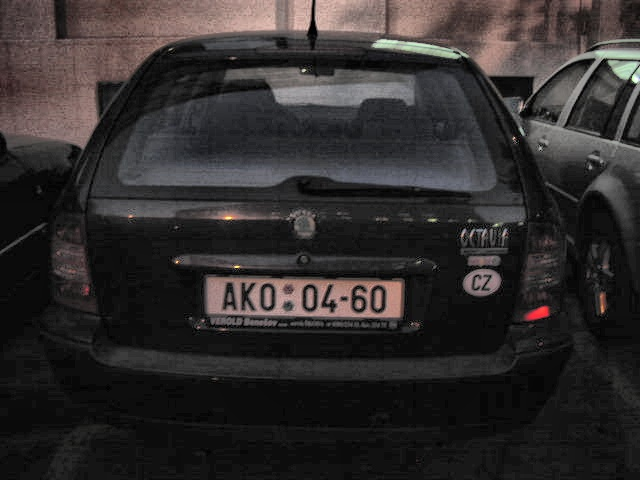
\includegraphics[width=\textwidth]{figures/ce_examples/2/clahe.jpg}
         \caption{Tamniji primjer uz jači kontrast}
     \end{subfigure}\\[0.5cm]
     \begin{subfigure}[b]{0.4\textwidth}
         \centering
         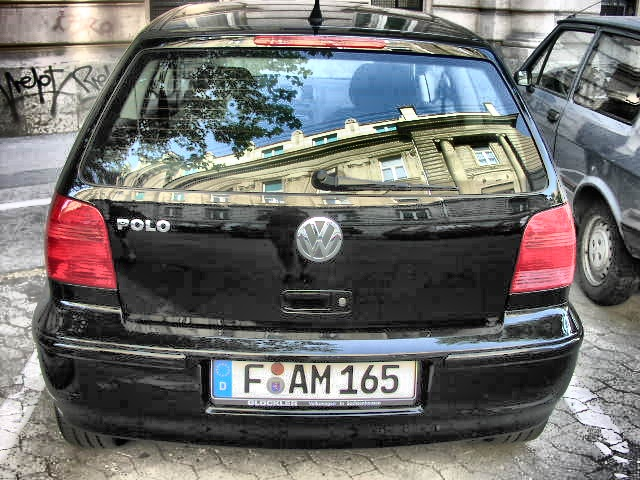
\includegraphics[width=\textwidth]{figures/ce_examples/3/clahe.jpg}
         \caption{Svjetliji primjer}
         \label{fig:ce_clahe_svijetli}
     \end{subfigure}
     \hspace{1cm}
     \begin{subfigure}[b]{0.4\textwidth}
         \centering
         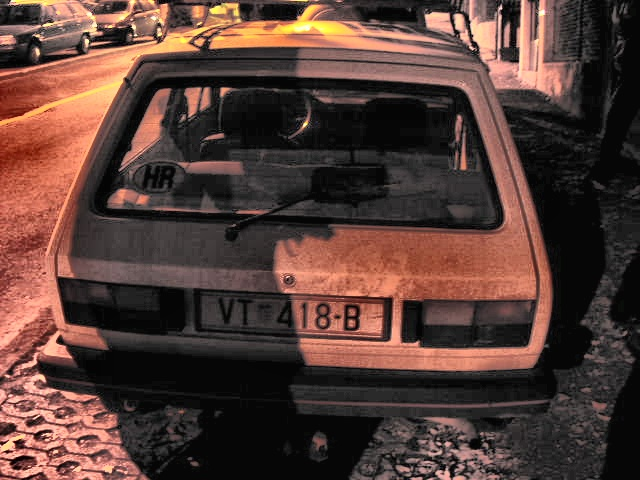
\includegraphics[width=\textwidth]{figures/ce_examples/4/clahe.jpg}
         \caption{Primjer sa sjenom}
         \label{fig:ce_clahe_sjena}
     \end{subfigure}
        \caption{Primjena algoritma CLAHE nad komponentom Y}
        \label{fig:ce_clahe}
\end{figure}

\subsection{Gaussov filter}
Kao što je već ranije rečeno, kako bi umanjili utjecaj šuma na slikama, potrebno je iskoristiti neku vrstu filtera nad istom. Razlikujemo linearne i nelinearne filtere. Obje vrste djeluju nad nekakvim manjim susjedstvom baš kao i algoritam CLAHE, a glavna razlika navedenih je u tome što je utjecaj linearnih uvijek jednak nad svakim susjedstvom, dok nelinearni djeluju dinamično. Za linearne vrijedi formulacija:
\begin{equation}
    F(A+B) = F(A) + F(B),
\end{equation}
gdje su $A$ i $B$ primjeri ulaznih signala, dok je $F$ funkcija linearnog filtera. Također, linearni filteri se definiraju pomoću matematičke operacije konvolucija. O istoj ćemo reći nešto više kasnije kada se dotaknemo konvolucijskih neuronskih mreža, a do tada, na jednoj apstraktnoj razini i primjeni u obradi slika, konvolucija je ništa drugo nego klizeći prozor pomoću kojeg se intenziteti piksela mijenjaju na temelju težinske sume klizećeg prozora i susjedstva originalne slike koji navedeni prozor definira. Važno je napomenuti da iako se za određivanje novog intenziteta promatra cijelo susjedstvo, promjena se primjenjuje samo na centralni piksel prozora i trenutnog susjedstva. Kako bi navedeno bilo primjenjivo nad svakim pikselom originalne slike te s obzirom na to da se svaki piksel točno jednom mora nalaziti u centru susjedstva, potrebno je sliku nadopuniti određenim okvirima u oba smjera kako bi matematika filtera funkcionirala. Postoje razne tehnike nadopunjavanja koje ćemo spomenuti kasnije.

Glavni primjer nelinearnog filtera je medijan filter koji u zadanom susjedstvu svaki centralni piksel zamjenjuje s medijan vrijednosti tog susjedstva. Svako susjedstvo u većini slučajeva ima različitu vrijednost medijana te upravo to potkrepljuje dinamičnost takvih filtera i u ovom radu takva vrsta filtera nije razmatrana. Kao primjer linearnog filtera razmatran je Gaussov filter koji je definiran sljedećom funkcijom:
\begin{equation}
    G(x,y) = \frac{1}{2\pi\sigma_x\sigma_y}e^{-(\frac{x^2}{2\sigma_x^2} + \frac{y^2}{2\sigma_y^2})},
    \label{eq:gauss_two_sigmas}
\end{equation}
gdje $(x,y)$ predstavlja poziciju u definiranom filteru, a $\sigma_x$ i $\sigma_y$ predstavljaju standardnu devijaciju u smjeru $x$, odnosno smjeru $y$. U većini slučajeva su vrijednosti navedenih standardnih devijacija jednake, pa se izraz \ref{eq:gauss_two_sigmas} pojednostavljuje u sljedeći izraz:
\begin{equation}
    G(x,y) = \frac{1}{2\pi\sigma^2}e^{-(\frac{x^2 + y^2}{2\sigma^2})}.
\end{equation}
Navedena formula je naravno u kontinuiranoj domeni, a nama je potrebna diskretna s obzirom na to da radimo sa slikama, stoga ju je potrebno aproksimirati. Nećemo ulaziti u detalje kako se to izvodi, ali ćemo prikazati jedan primjer. Sljedeći izraz predstavlja aproksimaciju $3 \times 3$ Gaussovog filtera: 
\begin{equation}
    K\footnote{Filter je normaliziran tako da suma svih elemenata bude 1 kako bi intenzitet piksela ostao u validnom rasponu.} = \frac{1}{16}
    \begin{bmatrix}
        1 & 2 & 1 \\
        2 & 4 & 2 \\
        1 & 2 & 1
    \end{bmatrix}.
    \label{eq:gauss_approx}
\end{equation}
Što se tiče indeksiranja takvih filtera, pravilo je sljedeće: središnji element, a to je 4 u ovom slučaju, se nalazi na poziciji $(0,0)$, što znači da indeksiranje kreće od $(-1,-1)$ do $(1,1)$. Općenito, indeksiranje kreće od $(\lceil -size_x/2 \rceil, \lceil -size_y/2 \rceil)$ do $(\lfloor size_x/2 \rceil, \lfloor size_y/2 \rceil)$, gdje $size_x$ i $size_y$ predstavljaju broj elemenata u smjeru $x$, odnosno smjeru $y$ i često su te dvije vrijednosti jednake.

Sve navedeno jest odlika filtera koji se koriste u operaciji konvolucija, no glavna razlika regularne konvolucije koja se npr.\ koristi u konvolucijskim neuronskim mrežama i konvolucije koja se koristi u raznim linearnim filterima za obradu slike je u tome što se prvo mora učiti dok je drugo uvijek poznato.

Na slici \ref{fig:ce_gauss} je prikazana primjena Gaussovog filtera\footnote{Veličina filtera je $3 \times 3$ i $\sigma=0.8$.} nakon algoritma CLAHE nad komponentom Y. Možda se golim okom utjecaj istog ne vidi najbolje, ali zasigurno on postoji i računalu bitno olakšava raspoznavanje u narednim koracima sustava. Ovako procesirane slike se dalje šalju u algoritam za pronalaženje područja interesa kojeg obrađujemo u sljedećoj sekciji.

\subsection{Konverzija RGB u nijanse sive}
Prije nego krenemo na sljedeći korak sustava, potrebno je spomenuti još jednu vrlo korištenu konverziju prostora boja, a to je konverzija iz prostora boja RGB u prostor boja nijansi sive. Taj prostor je jako koristan kada je potrebno učiti duboke modele jer se broj parametara smanjuje za tri puta s obzirom na to da se broj kanala smanjuje s tri na jedan. Konverzija je definirana na sljedeći način\footnote{https://docs.opencv.org/4.x/de/d25/imgproc\_color\_conversions.html}:
\begin{equation}
    Y \leftarrow 0.299 \cdot R + 0.587 \cdot G + 0.114 \cdot B,
\end{equation}
\begin{equation}
    R \leftarrow Y, G \leftarrow Y, B \leftarrow Y.
\end{equation}
Ovaj korak je korišten nakon što su sva područja interesa pronađena kako bi iste pripremili za duboke modele.

\begin{figure}[H]
     \centering
     \begin{subfigure}[b]{0.4\textwidth}
         \centering
         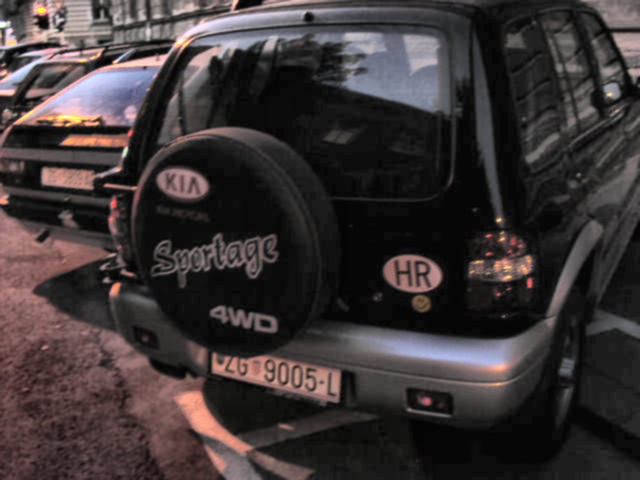
\includegraphics[width=\textwidth]{figures/ce_examples/1/gauss.jpg}
         \caption{Tamniji primjer}
         \label{fig:ce_gauss_tamniji}
     \end{subfigure}
     \hspace{1cm}
     \begin{subfigure}[b]{0.4\textwidth}
         \centering
         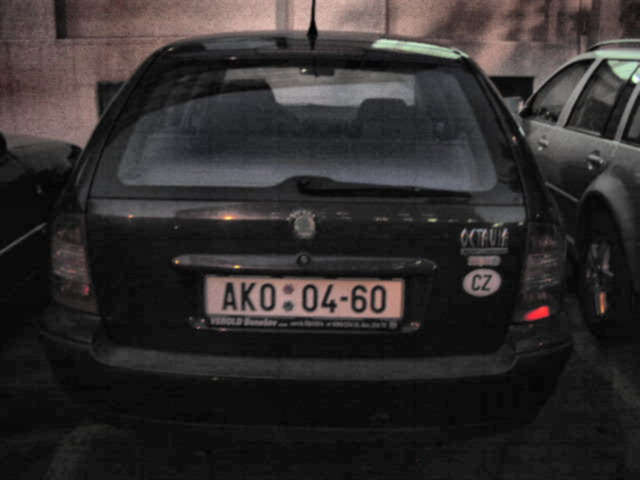
\includegraphics[width=\textwidth]{figures/ce_examples/2/gauss.jpg}
         \caption{Tamniji primjer uz jači kontrast}
     \end{subfigure}\\[0.5cm]
     \begin{subfigure}[b]{0.4\textwidth}
         \centering
         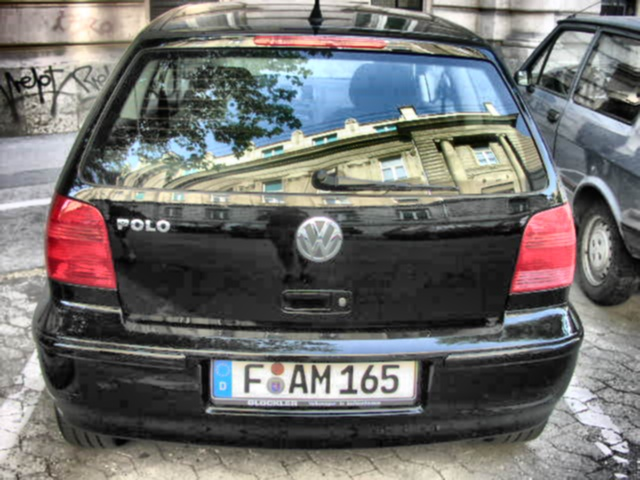
\includegraphics[width=\textwidth]{figures/ce_examples/3/gauss.jpg}
         \caption{Svjetliji primjer}
     \end{subfigure}
     \hspace{1cm}
     \begin{subfigure}[b]{0.4\textwidth}
         \centering
         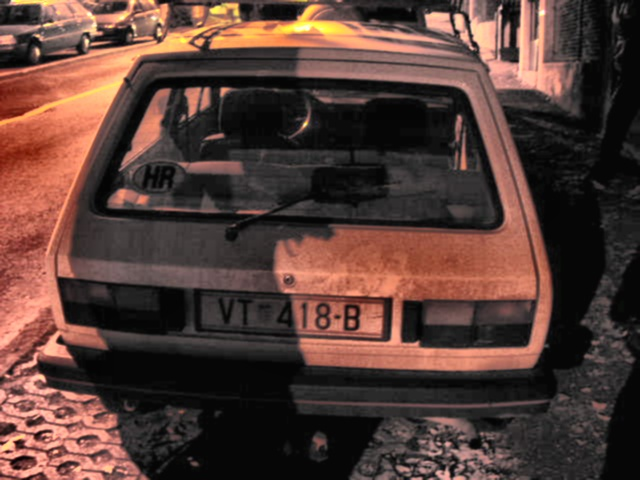
\includegraphics[width=\textwidth]{figures/ce_examples/4/gauss.jpg}
         \caption{Primjer sa sjenom}
     \end{subfigure}
        \caption{Primjena Gaussovog filtera nakon algoritma CLAHE nad komponentom Y}
        \label{fig:ce_gauss}
\end{figure}

\section{Pronalaženje područja interesa}
Algoritam za pronalaženje područja interesa je, kao što je već nekoliko puta rečeno, možda i najbitniji korak u sustavu za detekciju objekata. Potrebno je u vrlo kratkom vremenu pronaći veliki broj područja koji pokrivaju potencijalne objekte. Postavlja se pitanje na koji način to efikasno izvesti, kako uopće ocijeniti je li nešto objekt ili je možda to nešto dio nekog drugog objekta. Problem pronalaska takvih područja naziva se segmentacija \engl{segmentation}, a algoritmi koji rješavaju probleme segmentacije slika nazivaju se algoritmi superpiksela \engl{superpixel algorithms}. Ideja je da se slika podijeli na područja varijabilnih veličina koja bi kao grupa piksela predstavljala nešto smislenije nego kada bi se promatrao piksel po piksel. To je i logično jer piksel sam za sebe nam ne predstavlja ništa i na temelju jednog piksela nije moguće donijeti nikakvu razumnu odluku. U ovome radu se ne bavimo detaljima navedenih algoritama, već ih koristimo kao početni korak za neki drugi algoritam koji se bavi pronalaskom područja interesa. Više o navedenom se može pronaći u \citep{slic-paper}.

Jedan od prvih pristupa problemu pronalaska područja interesa bilo je korištenje klizećeg prozora \engl{sliding window} i piramide slike \engl{image pyramid}\footnote{Zanimljive animacije se mogu pronaći na sljedećoj poveznici: https://pyimagesearch.com/2015/03/23/sliding-windows-for-object-detection-with-python-and-opencv/}. Ideja je da se izabere određena veličina klizećeg prozora koji će zatim prolaziti kroz sliku uz određeni korak. Područje koje se nalazi pod trenutnom pozicijom klizećeg prozora se transformira u određeni skup značajki te se zatim klasificira prethodno naučenim klasifikatorom. Najčešći primjer navedenog je kombinacija HOG značajki i SVM-a. Kako objekti na slici mogu biti raznih dimenzija, klizeći prozor konstantnih dimenzija nije u stanju kvalitetno izdvojiti sva željena područja. Problem se rješava tako da se koristi piramida slike. Piramida slike je ništa drugo nego skup slika koje nastaju iz originalne slike smanjivanjem veličine \engl{downscale} iste do predefinirane vrijednosti. Često taj faktor skaliranja iznosi 2, što znači da se svaka sljedeća slika dobije tako da se prethodnoj slici veličina smanji 2 puta. Tako prethodno definirani prozor može obuhvatiti različite omjere veličina objekata.

Navedeni primjer je primjer iscrpne pretrage \engl{exhaustive search} koji bi u teoriji trebao biti najpouzdaniji jer se pametnim izborom parametara veličine klizećeg prozora i veličina slika može obuhvatiti gotovo sve moguće kombinacije objekata i omjera njihovih veličina. No u praksi se takav pristup izbjegava u širokom luku i razlog za to je vrlo očigledan. Algoritam je vrlo spor i izrazito računski zahtjevan. Dakle, ideja je pronaći algoritam koji će biti znatno efikasniji od prethodnog, koji će sva područja, koji potencijalno sadrže objekte, bez dvojbe pronaći neovisno o omjeru veličine slike i samog objekta na istoj i koji će se maknuti od ideje klizećeg prozora i prolaska istog po slici. Jedan od boljih algoritama koji rješava navedenu problematiku je Selektivno pretraživanje kojeg ćemo obraditi u nastavku.

\subsection{Selektivno pretraživanje}
Selektivno pretraživanje \engl{selective search} je jedan od revolucionarnijih algoritama za pronalaženje područja interesa. Znatno je memorijski i računski efikasniji nego ranije navedeni algoritam klizećeg prozora i piramide slike jer u svojem temelju za generiranje početnih područja koristi jedan od efikasnijih algoritama segmentacije čije rezultate zatim hijerarhijski grupira na temelju pet mjera sličnosti: sličnost boja \engl{colour similarity}, sličnost tekstura \engl{texture similarity}, sličnost veličina \engl{size similarity}, sličnost oblika \engl{shape similarity} i meta sličnost \engl{meta similarity}. Radi se o aglomerativnom tipu hijerarhijskog algoritma grupiranja \engl{hierarchical agglomerative clustering, HAC} kod kojeg je broj početnih grupa jednak broju primjera koje zatim iterativno grupira na temelju neke mjere sličnosti sve dok cijela slika ne postane jedna velika grupa. Radi se o tzv.\ pristupu \textit{bottom-up}. U nastavku se nalazi pseudokod navedenog algoritma.

\begin{algorithm}[h]
    \caption[Caption for LOF]{Algoritam HAC\footnotemark}
    \label{alg:hac}
    \SetAlgoLined
    \Input{Slika (u boji)}
    \Output{Skup hipoteza $L$ o lokacijama objekata}
    \bigskip
    Generiraj početna područja $R = \{r_1, \dots , r_n\}$ pomoću \citep{Felzenszwalb2004}\;
    Inicijaliziraj skup sličnosti $S = \emptyset$\;
    \ForEach{\textit{Par susjednih područja} $(r_i,r_j)$}{
        Izračunaj sličnost $s(r_i,r_j)$\;
        $S = S \cup s(r_i,r_j)$\;
    }
    \While{$S \ne \emptyset$}{
        Dohvati najveću sličnost $s(r_i,r_j) = \max(S)$\;
        Spoji odgovarajuća područja $r_t = r_i \cup r_j$\;
        Ukloni sličnosti vezane uz $r_i : S = S \setminus s(r_i,r_*)$\;
        Ukloni sličnosti vezane uz $r_j : S = S \setminus s(r_*,r_j)$\;
        Izračunaj skup sličnosti $S_t$ između $r_t$ i njegovih susjeda\;
        $S=S \cup S_t$\;
        $R=R \cup r_t$\;
    }
    Izdvoji lokacije objekata $L$ iz svih područja skupa $R$\;
\end{algorithm}
\footnotetext{Prilagođeno iz \citep{ss-paper}.}

Algoritam koji pronalazi parove susjednih područja nije naveden u radu, ali logično je za pretpostaviti da se radi o vrlo jednostavnom algoritmu koji provjerava dodiruju li se generirana područja ili preklapaju.

Glavna ideja samog pristupa je pokušati pronaći razne strategije diversifikacije \engl{diversification strategies} koje će rezultirati robusnijim algoritmom. Pored navedenih komplementarnih mjera sličnosti \engl{complementary similarity measures}, to se postiže i provođenjem algoritma u raznim komplementarnim prostorima boja \engl{complementary colour spaces} poput HSV, RGB, Lab itd.\ , ovisno o verziji samog algoritma te s brojnim komplementarnim početnim područjima \engl{complementary starting regions}. Postoje tri verzije algoritma: \textit{single}, \textit{fast} i \textit{quality}. Svaka verzija se razlikuje u broju korištenih strategija diversifikacije, pa tako verzija \textit{single} koristi 1 strategiju, verzija \textit{fast} 8 strategija i verzija \textit{quality} 80 strategija. Naravno, što je broj strategija veći, to je krajnji rezultat bolji, ali istovremeno je računski i vremenski skuplje. U \citep{ss-paper} se iznosi određena statistika koja prikazuje kako izvedba verzije \textit{single} traje 0.71s, verzije \textit{fast} 3.79s i verzije \textit{quality} 17.15s. Navedena vremena su prikazana okvirno, jer brzina dosta ovisi o specifikacijama računala, ali bitno je uočiti razlike među verzijama. U konačnom sustavu je korištena verzija \textit{fast} koja je relativno brza i daje solidne rezultate.

Algoritam na kraju prvo vraća one lokacije objekata za koje je izrazito siguran da su stvarno objekti. Kako bi se smanjila pristranost \engl{bias} prema velikim područjima, korišten je nedeterminizam u kojem se sva područja rangiraju na sljedeći način:
\begin{equation}
    v_i^j = RND \times i,    
\end{equation}
gdje $v_i^j$ predstavlja rang i-tog generiranog područja j-te strategije, a $RND$ predstavlja slučajan broj iz $[0,1]$. Jednom kada su svi rangovi izračunati, mogući duplikati nižeg ranga se brišu, a ostali se sortiraju po vrijednosti ranga. 

Na slici \ref{fig:ss} se nalazi primjer rada selektivnog pretraživanja. Jasno se vidi kako se hijerarhija područja gradi iterativno sve dok slika ne postane potencijalno jedna grupa. U nastavku ćemo dati kratak osvrt na algoritam koji generira inicijalna područja i na mjere sličnosti. Ostali detalji se mogu pronaći u izvornom radu \citep{ss-paper}.

\begin{figure}[H]
    \centering
    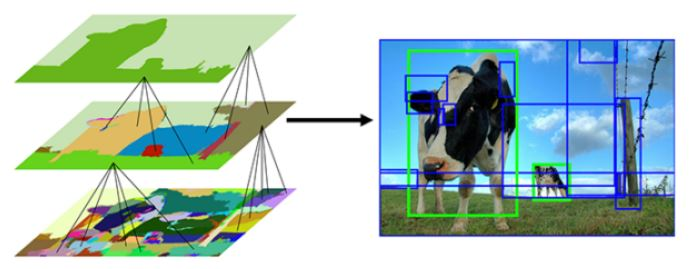
\includegraphics[scale=0.75]{figures/detector/ss.jpg}
    \caption[Caption for LOF]{Rezultat selektivnog pretraživanja\footnotemark}
    \label{fig:ss}
\end{figure}
\footnotetext{https://pyimagesearch.com/2020/06/29/opencv-selective-search-for-object-detection/}

\subsubsection{Algoritam Felzenszwalb}
Algoritam koji se bavi segmentacijom početnih područja je učinkovita segmentacija slike temeljena na grafovima \engl{efficient graph-based image segmentation} poznatije u literaturi kao algoritam Felzenszwalb \engl{Felzenszwalb's algoritam}. Na slici \ref{fig:ss} s lijeve strane prva slika od tri predstavlja rezultat promatranog algoritma. Zadaća algoritma je pomoću teorije grafova na slici segmentirati ona područja koja sadržavaju potencijalne objekte. Želja samih autora algoritma je da naprave takav pristup koji će moći biti korišten za mnoštvo različitih problema računalnog vida baš kao što se i detektiranje rubova \engl{edge detection} koristi. Da bi to bilo izvedivo, algoritam mora zadovoljavati sljedeće: obuhvaćanje perceptivno važnih grupacija ili područja koja često odražavaju globalne aspekte slike i linearna vremenska kompleksnost u ovisnosti o broju piksela \citep{Felzenszwalb2004}.

Kao početni korak potrebno je sliku pretvoriti u neusmjereni težinski graf \engl{undirected weighted graph} $G = (V,E)$ s vrhovima \engl{vertices} $v_i \in V$ i bridovima \engl{edges} $(v_i, v_j) \in E$, gdje $(v_i,v_j)$ predstavlja brid između vrha $v_i$ i vrha $v_j$. Svaki brid posjeduje određenu težinu $w((v_i,v_j))$ koja predstavlja nenegativnu mjeru različitosti \engl{dissimilarity measure} između dva susjedna vrha $v_i$ i $v_j$. U slučaju segmentacije slika, vrhovi su zapravo pikseli, dok je težina bridova mjera različitosti između dva piksela temelja npr.\ na intenzitetu, boji, lokaciji i sl. Konačni cilj algoritma je dobiti segmentaciju $S$ grafa $G$ tako da vrijedi $G^{'} = (V, E^{'})$, gdje $E^{'} \subset E$. $S$ dijeli $G$ u $G^{'}$ tako da sadrži različite komponente \engl{distinct components} $C$. U izvornom radu \citep{Felzenszwalb2004} su promatrana dva načina generiranja grafova: generiranje temeljeno na fizičkom susjedstvu od 8 piksela nazvano rešetkasti graf \engl{grid graph} te generiranje temeljeno na najbližem susjedstvu nazvano graf najbližeg susjedstva \engl{nearest neighbor graph}. Mjera različitosti rešetkastog grafa definirana je kao apsolutna razlika između intenziteta piksela. Kod grafa najbližeg susjedstva, svaki piksel je jedna točka u prostoru značajki $(x,y,r,g,b)$, gdje $(x,y)$ predstavlja fizičku lokaciju piksela, a $(r,g,b)$ vrijednost boje. Prostor boja ne mora nužno biti RGB, već može biti i neki drugi. Mjera različitosti grafa najbližeg susjedstva je onda definirana kao $L_2$ norma razlike dvije točke, a broj promatranih susjeda je 10.

Nakon što je faza generiranja grafa završena, slijedi faza segmentacije ili, u žargonu teorije grafova, particioniranje grafa. Kriterij \engl{predicate} koji određuje jesu li određene komponente neovisne \engl{independent} jedna o drugoj definiran je na sljedeći način:
\begin{equation}
    D(C_1,C_2) =
    \begin{cases}
        \mbox{Da,} & \mbox{ako }Dif(C_1,C_2) > MInt(C_1,C_2) \\
        \mbox{Ne,} & \mbox{inače}
    \end{cases},
\end{equation}
gdje $Dif(C_1,C_2)$ predstavlja razliku između dvije komponente, a $MInt(C_1,C_2$ najmanja unutarnju razliku između dvije komponente.

Razlika između dvije komponente je definirana na sljedeći način:
\begin{equation}
    Dif(C_1,C_2) = \min_{v_i \in C_1, v_j \in C_2, (v_i,v_j) \in E} w(v_i,v_j).
\end{equation}
U slučaju da brid između dvije komponente ne postoji, onda vrijedi $Dif(C_1,C_2) = \infty$. Dakle, razlika između dvije komponente je ništa drugo nego najmanja težina brida koji spaja iste.

Najmanja unutarnja razlika između dvije komponente definirana je na sljedeći način:
\begin{equation}
    MInt(C_1,C_2) = \min(Int(C_1) + \tau(C_1), Int(C_2) + \tau(C_2)).
\end{equation}
$Int(C)$ predstavlja unutarnju razliku komponente definirane na sljedeći način:
\begin{equation}
    Int(C) = \max_{e \in MST(C,E)} w(e),
\end{equation}
gdje $MST$ predstavlja najmanje razapinjuće stablo \engl{minimum spanning tree}.
Intuicija iza navedene mjere je ta da komponenta $C$ ostaje povezana samo ako se promatraju bridovi težina barem $Int(C)$. Dakle, unutarnja razlika komponente je ništa drugo nego najveća težina brida koji spaja dva vrha iste. $\tau(C)$ predstavlja funkciju praga \engl{threshold function} definirane na sljedeći način:
\begin{equation}
    \tau(C) = \frac{k}{|C|},
\end{equation}
gdje $|C|$ predstavlja veličinu komponente $C$, a $k$ pozitivnu konstantu. Funkcija praga pomaže pri ekstremnim slučajevima kada je $|C| = 1$ te pomaže kod određivanja mjere ranije navedenog kriterija. Kako $k$ raste, tako i sklonost prema većim komponentama raste. Također, parametar $k$ je dio strategija diversifikacije jer njegovim mijenjanjem se generiraju drugačija početna područja.

Na slici \ref{fig:partitioning} se nalazi jedan primjer particioniranja grafa. Više detalja i prikaz primjera se može pronaći u izvornom radu \citep{Felzenszwalb2004}.
\begin{figure}[H]
    \centering
    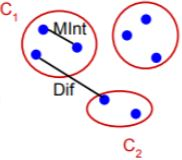
\includegraphics[scale=0.8]{figures/detector/felzenszwalb.jpg}
    \caption[Caption for LOF]{Primjer particioniranja\footnotemark}
    \label{fig:partitioning}
\end{figure}
\footnotetext{Ostatak zanimljivih primjera se može pronaći na sljedećoj poveznici: https://www.analyticsvidhya.com/blog/2021/05/image-segmentation-with-felzenszwalbs-algorithm/}

\subsubsection{Sličnost boja}
Za svako područje $r_i$ se konstruira histogram boje kroz sve kanale koristeći 25 pretinaca \engl{bins}. To rezultira histogramom boja $C_i = \{c_i^1, \dots , c_i^n\}$ područja $r_i$ dimenzionalnosti $n=75$ kada se koriste tri kanala boje. Histogrami se zatim normaliziraju pomoću $L_1$ norme. Sličnost boja se onda računa kao presjek histograma:
\begin{equation}
    s_{colour}(r_i,r_j) = \sum_{k=1}^{n}\min(c_i^k,c_j^k).
\end{equation}
Zgodna stvar je što se jednom izračunati histogrami vrlo lako mogu propagirati kroz hijerarhiju, pa ih nije potrebno iznova konstruirati prilikom spajanja dva područja. To se postiže na sljedeći način:
\begin{equation}
    C_t = \frac{\text{size}(r_i) \times C_i + \text{size}(r_j) \times C_j}{\text{size}(r_i) + \text{size}(r_j)},
\end{equation}
gdje se veličina novog područja računa kao suma dva prethodna:
\begin{equation}
    \text{size}\footnote{Predstavlja veličinu područja u pikselima.}(r_t) = \text{size}(r_i) + \text{size}(r_j).
\end{equation}

\subsubsection{Sličnost tekstura}
Tekstura nekog područja $r_i$ se konstruira na temelju SIFT značajki koje ne obrađujemo u ovom radu, no detalji se mogu pronaći u \citep{sift-paper} i \citep{szeliski}. Ne koriste se SIFT značajke kao takve, već se konceptualno primjenjuje ideja iza istih. Dakle, za svaki kanal boje se konstruiraju Gaussove derivacije u osam orijentacija. Zatim se za svaki kanal boje i za svaku orijentaciju konstruira histogram tekstura koristeći 10 pretinaca. To rezultira histogramom tekstura $T_i = \{t_i^1, \dots , t_i^n\}$ područja $r_i$ dimenzionalnosti $n=240$ kada se koriste tri kanala boje. Histogrami se zatim normaliziraju pomoću $L_1$ norme. Sličnost tekstura se onda računa kao presjek histograma:
\begin{equation}
    s_{texture}(r_i,r_j) = \sum_{k=1}^{n}\min(t_i^k,t_j^k).
\end{equation}
Propagacija histograma tekstura kroz hijerarhije je identična propagaciji histograma boja. 

\subsubsection{Sličnost veličina}
Ideja ove sličnosti je da se manja područja puno brže spoje. To znači da bi područja skupa $S$ (\textit{i.e}.\ područja koja još nisu spojena s drugim područjima) trebala biti slične veličine kroz cijeli algoritam. Navedeni princip je poželjan jer tako lokacije objekata svih mogućih skala dolaze do izričaja. Također, sprječava se da velika područja preuzmu manja jedan po jedan. Sličnost veličina se računa na sljedeći način:
\begin{equation}
    s_{size}(r_i,r_j) = 1 - \frac{\text{size}(r_i) + \text{size}(r_j)}{\text{size}(im)},
\end{equation}
gdje $im$ predstavlja originalnu sliku.

\subsubsection{Sličnost oblika}
Ideja ove sličnosti je provjeriti koliko se dva područja $r_i$ i $r_j$ preklapaju. Ako se područje $r_i$ u potpunosti nalazi u području $r_j$, logično je takva područja spojiti. Također, ako se dva područja uopće ne preklapaju ili se vrlo malo preklapaju, onda ih vjerojatno nije pametno spojiti. Sličnost oblika se računa na sljedeći način:
\begin{equation}
    s_{fill}(r_i,r_j) = 1 - \frac{\text{size}(BB_{ij}) - \text{size}(r_i) - \text{size}(r_j)}{\text{size}(im)},
\end{equation}
gdje $BB_{ij}$ predstavlja granični okvir \engl{bounding box} oko područja $r_i$ i $r_j$. Navedena mjera sličnosti se također efikasno može izračunati kroz hijerarhije ako se čuvaju granični okviri oko inicijalnih područja.

\subsubsection{Meta sličnost}
Meta sličnost je kombinacija prethodno navedenih sličnosti:
\begin{equation}
    s(r_i,r_j) = a_1s_{colour}(r_i,r_j) + a_2s_{texture}(r_i,r_j) + a_3s_{size}(r_i,r_j) + a_4s_{fill}(r_i,r_j),
\end{equation}
gdje $a_i \in \{0,1\}$ predstavlja promatra li se trenutna mjera sličnosti ili ne.

\section{Klasifikacija područja interesa}
Nakon što su područja interesa pronađena, slijedi faza prepoznavanja istih i klasifikacija pripada li pronađeno područje skupu registarskih tablica ili ne pripada. Kao što je rečeno u uvodu ovog velikog poglavlja, da bi sustav za detekciju registarskih tablica bio otporan na lažno pozitivne primjere koji nastaju vrlo pohlepnim načinom pronalaska istih poput običnih detekcija linija, potrebno je naučiti model strojnog učenja koji će biti u stanju vrlo efikasno odlučiti radi li se o registarskoj tablici ili ne. Također, kroz rad su navedeni neki od tipova mogućih značajki poput HOG, SIFT, Haar, koje vrlo dobro mogu reprezentirati objekte na slikama i koje u kombinaciji s klasičnim algoritmima strojnog učenja kao npr.\ SVM mogu rezultirati dosta kvalitetnim sustavom za detekciju. Danas se navedeni pristup sve manje i manje koristi upravo zbog pojave konvolucijskih neuronskih mreža koje generiraju puno kvalitetniju reprezentaciju objekata na slikama.

Sustav za detekciju registarskih tablica u ovom radu baziran je na \citep{rcnn-paper}. Navedeni rad za probleme detekcije objekata \engl{object detection} predlaže pristup u kojem se pomoću selektivnog pretraživanja pronalaze područja interesa koja se zatim predaju u konvolucijsku neuronsku mrežu koja generira skup značajki za svako predano područje. Tako generirane značajke se zatim predaju u binarni klasifikator SVM kako bi se odredilo pripada li navedeno područje skupu registarskih tablica ili ne pripada i u model linearne regresije za generiranje graničnog okvira. Dakle, za svaku sliku se pronalazi oko 2000\footnote{Selektivno pretraživanje može generirati i nekoliko tisuća područja koja naravno nije sva potrebno provjeravati.} područja interesa i svako od tih područja prolazi kroz konvolucijsku neuronsku mrežu, binarni klasifikator i model linearne regresije. U literaturi se navedeni pristup često naziva konvolucijska neuronska mreža temeljena na regiji \engl{region-based convolutional neural network, R-CNN}.

Sve skupa navedeno je dosta sporo s obzirom na broj promatranih područja interesa i na brzinu selektivnog pretraživanja, ali pruža dobar osnovni pristup \engl{baseline approach} u problemima detekcije objekata. U ovom radu je pristup malo pojednostavljen jer se ne koristi SVM kao binarni klasifikator, nego jednostavna unaprijedna potpuno povezana neuronska mreža \engl{feedforward fully-connected neural network} i ne koristi se model linearne regresije za predviđanje graničnog okvira, već se granični okvir preuzima od selektivnog pretraživanja i ne modificira se. Na slici \ref{fig:rcnn} je prikazan hodogram R-CNN arhitekture bez prisustva modela linearne regresije.

\begin{figure}[H]
    \centering
    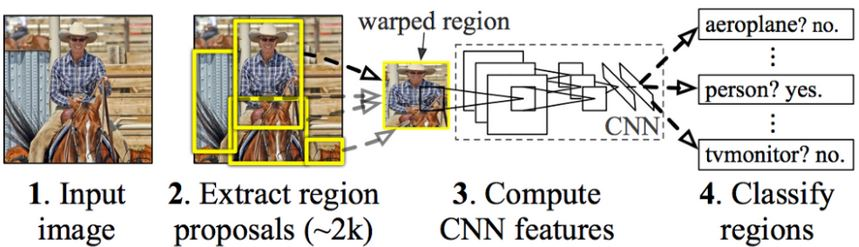
\includegraphics[scale=0.5]{figures/detector/rcnn.jpg}
    \caption[Caption for LOF]{Hodogram R-CNN arhitekture\footnotemark}
    \label{fig:rcnn}
\end{figure}
\footnotetext{Oznake na slici su na engleskom jeziku jer je slika preuzeta iz izvornog rada, no one opisuju pravo sve dosad rečeno.}

Svaki algoritam strojnog učenja analiziramo u smislu tri glavne komponente: model, funkcija gubitka i optimizacijski postupak. Optimizacijskih postupaka ima mnogo, no kada je riječ o neuronskim mrežama, onda se koriste algoritmi temelji na gradijentima \engl{gradient-based algorithms}. U ovom radu nećemo detaljno obrađivati navedene, već ćemo u poglavlju o rezultatima cjelokupnog sustava dati kratak osvrt koji algoritam je korišten i zašto. S obzirom na to da model sustava za detekciju registarskih tablica ovisi o značajkama koje generira konvolucijska neuronska mreža, prvo ćemo dati kratak osvrt o istoj, a zatim ćemo opisati model sustava za detekciju registarskih tablica, funkciju gubitka i kako su ulazni podaci generirani.

\subsection{Konvolucijske neuronske mreže}
Konvolucijska neuronska mreža \engl{convolutional neural network, CNN} je tip neuronske mreže koja je specijalizirana za obradu podataka rešetkaste \engl{grid-like} topologije \citep{Goodfellow-et-al-2016}. Neki od primjera u 1-D svijetu je npr.\ promatranje EKG signala kroz fiksne vremenske intervale i takvu primjenu ne promatramo u ovom radu, a u 2-D svijetu promatranje slika zbog primjene u npr.\ detekciji objekata. Samo ime nalaže da se u strukturi konvolucijske neuronske mreže upotrebljava matematička operacija konvolucija koju smo spomenuli kratko iz perspektive obrade slike.

Konvolucija u diskretnoj domeni nad slikom je definirana na sljedeći način:
\begin{equation}
    S(i,j) = (I \ast K)(i,j) = \sum_{m}\sum_{n}I(m,n)K(i-m,j-n),
\end{equation}
gdje su $i$ i $j$ pozicije piksela na slici $I$, a $K$ jezgra \engl{kernel} ili filter veličine $m \times n$. Rezultat se u literaturi često naziva mapa značajki \engl{feature map}. Konvolucija je komutativna \engl{commutative} pa možemo pisati i sljedeće:
\begin{equation}
    S(i,j) = (K \ast I)(i,j) = \sum_{m}\sum_{n}I(i-m,j-n)K(m,n).
\end{equation}
Ovo svojstvo je zgodno kod dokazivanja matematičkih teorema, no kod implementacije neuronskih mreža i nije toliko bitno. Često se kod implementacije neuronskih mreža koristi unakrsna korelacija \engl{cross-correlation} koja je definirana na sljedeći način:
\begin{equation}
    S(i,j) = (K \ast I)(i,j) = \sum_{m}\sum_{n}I(i+m,j+n)K(m,n)
\end{equation}
jer algoritmu strojnog učenja nije bitno je li indeksiranje jezgre okrenuto kada će naučiti one vrijednosti koje su u tom trenutku najbolje. Iako se radi o korelaciji, mnoge implementacije ju nazivaju i konvolucijom zbog jednostavnosti i sličnosti jedne s drugom.

Konvolucijska neuronska mreža donosi tri bitna svojstva kako bi poboljšala nedostatke koje unaprijedna potpuno povezana neuronska mreža ima kada je riječ o slikama, a to su rijetke interakcije \engl{sparse interactions}, dijeljenje parametara \engl{parameter sharing} i ekvivalentna reprezentacija \engl{equivariant representation}. Ukratko, rijetke interakcije smanjuju broj veza između ulaznih i izlaznih neurona, ovisno o broju jezgri konvolucija. Kod unaprijedne potpuno povezane neuronske mreže gdje postoji $n$ ulaza i $m$ izlaza, vremenska složenost iznosi $O(n \times m)$, dok kod konvolucijske neuronske mreže iznosi $O(n \times k)$, gdje $k$ predstavlja broj konekcija izlaza. Dijeljenje parametara je možda najveći skok u odnosu na unaprijednu potpuno povezanu neuronsku mrežu jer kod iste se svaki parametar koristi točno jednom za svaki primjer, dok se kod konvolucijske neuronske mreže ti parametri dijele tako da jezgra konvolucije prolazi po slici koristeći iste parametre za različite lokacije pa se time smanjuje broj parametara i do nekoliko stotina puta. Upravo je to princip superpiksela, što smo spomenuli ranije. Ekvivalentnost funkcije znači da ako se ulaz promijeni na neki način, izlaz se mijenja na isti način. Matematički rečeno: funkcija $f(x)$ je ekvivalentna funkciji $g$ ako $f(g(x)) = g(f(x))$. Konvolucija je npr.\ ekvivalentna s operacijom translacije \engl{translation}. Jedan od primjera koji to potvrđuje je detekcija rubova koja se događa pri prvim slojevima konvolucijske neuronske mreže. Jednom tako naučena reprezentacija se vrlo lako propagira u daljnje slojeve gdje se detekcija rubova događa praktički instantno zbog svih dosad navedenih svojstava \citep{Goodfellow-et-al-2016}.

\begin{figure}[H]
    \centering
    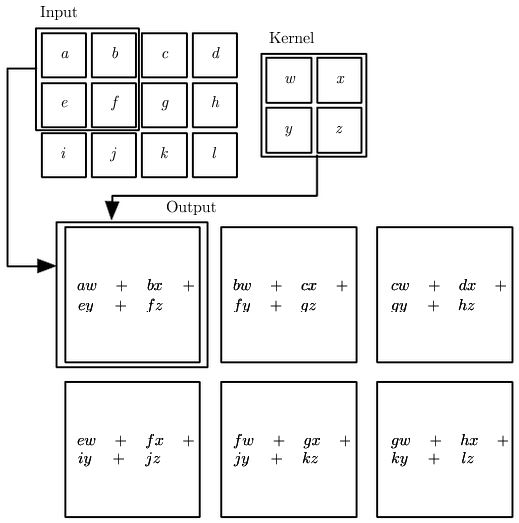
\includegraphics[scale=0.5]{figures/detector/conv.jpg}
    \caption[Caption for LOF]{Primjer konvolucije bez nadopunjavanja uz pomak 1\footnotemark}
    \label{fig:conv}
\end{figure}
\footnotetext{Preuzeto iz \citep{Goodfellow-et-al-2016}.}

Na slici \ref{fig:conv} nalazi se primjer kako konvolucija djeluje na jedan manji segment. Jezgra prolazi slikom i svaki prvi piksel zamjenjuje težinskom sumom susjedstva i jezgre. Primjer je možda malo neobičan s obzirom na parnu veličinu jezgre. U praksi to često i nije slučaj jer kada je jezgra parne veličine, gubi se simetrija koja se postiže neparnom veličinom. Najčešći primjeri su jezgre kvadratnih veličina $3 \times 3$ i $5 \times 5$ iako ni pravokutne kombinacije nisu isključene kao što ćemo vidjeti u nastavku. Uz veličinu jezgre, bitno je spomenuti hiperparametre pomak \engl{stride} i nadopunjavanje \engl{padding}. Pomak je ništa drugo nego koliko će se jezgra konvolucije kretati po slici u oba smjera. Veličina pomaka je isto najčešće kvadratna i iznosi $1 \times 1$ ili $2 \times 2$, ovisno o primjeni. Nadopunjavanje određuje kako postupiti kada jezgra konvolucije izlazi iz okvira slike kao što smo spomenuli kod Gaussovog filtera. Postoji nekoliko taktika poput nadopunjavanje nekom predefiniranom konstantom\footnote{Često se koristi 0.}:
\[iiiiii|abcdefgh|iiiiiii,\]
nadopunjavanje replikacijom:
\[aaaaaa|abcdefgh|hhhhhhh,\]
nadopunjavanje refleksijom:
\[fedcba|abcdefgh|hgfedcb,\]
nadopunjavanje refleksijom gdje se ignorira prvi element, tzv.\ refleksija 101:
\[gfedcb|abcdefgh|gfedcba\]
i mnoge druge \citep{szeliski}. U krajnjem sustavu za jezgre konvolucijskih neuronskih mreža se koristi nadopunjavanje nulama, dok se kod Gaussovog filtera koristi refleksija 101.

Sloj konvolucijske neuronske mreže se sastoji od nekoliko različitih komponenti. Prvo se u paraleli izvode konvolucije kako bi se dobile linearne aktivacije, zatim se iste provlače kroz neku nelinearnu funkciju poput sigmoide ili zglobnice \engl{rectified linear unit, ReLU} i na kraju se nelinearni izlazi provlače kroz komponentu koja se naziva sloj sažimanja \engl{pooling layer}. Ideja sloja sažimanja je reprezentaciju učiniti nepromjenjivom \engl{invariant} u odnosu na male pomake u ulaznom prostru. Postoji nekoliko tipova sloja sažimanja poput sažimanje maksimalnom vrijednosti \engl{max-pooling}, srednjom vrijednosti \engl{average-pooling} i sl. Sloj sažimanja također koristi jezgre kao i kod konvolucije jedino što ovdje nije riječ o konvoluciji kao takvoj, već o običnom klizećem prozoru koji uz svoju veličinu također posjeduje i pomak i nadopunjavanje kao svoje hiperparametre.

Hiperparametri pomak i nadopunjavanje utječu na veličinu izlaza na sljedeći način:
\begin{equation}
    W_{out} = \lfloor \frac{W_{in} - size_x + 2 * padding_x}{stride_x} + 1 \rfloor,
\end{equation}
\begin{equation}
    H_{out} = \lfloor \frac{H_{in} - size_y + 2 * padding_y}{stride_y} + 1 \rfloor,
\end{equation}
gdje $W$ predstavlja širinu \engl{width} slike, $H$ visinu \engl{height} slike i $size_i$ broj elemenata jezgre u i-tom smjeru. Često sve vrijednosti u formuli vrijede za obje dimenzije kada se radi o kvadratnim veličina, no slika \ref{fig:conv} pokazuje i primjenu pravokutnih veličina.

Uz navedene konstrukte, postoji nešto što se naziva i sloj normalizacije \engl{batch normalization layer}. S obzirom na to da su kod optimizacijskih postupaka baziranih na gradijentima moguće pojave poput iščezavajućeg gradijenta \engl{vanishing gradient} i eksplodirajućeg gradijenta \engl{exploding gradient}, podatke koji putuju kroz slojeve je potrebno normalizirati tako da im srednja vrijednost \engl{mean} bude oko 0 i standardna devijacija \engl{standard deviation} oko 1 kako bi cijeli postupak optimizacije bio stabilniji.

Konvolucijske neuronske mreže se, kao i unaprijedne potpuno povezane neuronske mreže, uče algoritmom propagacije pogreške unatrag \engl{backpropagation algorithm}. Glavna razlika je, kao što smo i ranije rekli, u broju parametara koje je potrebno optimizirati.

Ovom radu nije cilj ulaziti u toliko detalja oko samih konvolucijskih neuronskih mreža s obzirom na to da postoji brojna literatura koja ulazi u srž. Dana je neka generalna slika, a ostale informacije mogu se pronaći u \citep{guide-cnn}, \citep{Goodfellow-et-al-2016} i \citep{szeliski}.

\subsection{Model sustava za detekciju}
Arhitektura konvolucijske neuronske mreže za izlučivanje značajki bazirana je na radu \citep{crnn-paper} uz neke modifikacije u broju mapa koje se generiraju zbog ograničenih računalnih resursa. Tablica \ref{tab:cnn} prikazuje konfiguraciju slojeva konvolucijske neuronske mreže kao i kako se veličina ulazne slike mijenja, dok tablica \ref{tab:linear} prikazuje arhitekturu i konfiguraciju klasifikatora. Većina toga je pisano na engleskom jeziku zbog lakše usporedbe s mnogim literaturama koje su također pisane na engleskom jeziku. Ukratko ćemo objasniti značenje svakih od slojeva kao i još nekih oznaka.

Primjena slojeva \textit{Convolution}, \textit{MaxPooling} i \textit{BatchNormalization} objašnjena je ranije. \textit{\#maps} predstavlja broj mapa značajki, $k$ veličinu jezgre, $s$ veličinu pomaka i $p$ veličinu nadopunjavanja. U slučaju kada piše samo jedan broj, onda se radi o kvadratnoj veličini. Dakle, $k:3$ je zapravo $3\times3$ itd.\ , dok kada piše 0, znači da je taj segment izostavljen, odnosno da se ne koristi. Veličina slike kao i veličine jezgri prvo predstavljaju visinu slike pa zatim širinu. Dakle, ulazna slika je slika nijansi sive visine 32 piksela i širine 100 piksela itd. Unutar svakog sloja konvolucije se koristi nelinearna aktivacijska funkcija ReLU. U slučaju da je prisutan i sloj normalizacije, onda se navedena aktivacijska funkcija koristi tek nakon provedbe sloja normalizacije. Sloj \textit{Linear} predstavlja potpuno povezani sloj jedne unaprijedne potpuno povezane neuronske mreže, gdje $in$ predstavlja broj ulaznih neurona, dok $out$ predstavlja broj izlaznih neurona. Sloj \textit{Dropout} je primjer regularizacijskog \engl{regularization} sloja koji s vjerojatnosti $p$ određuje hoće li se trenutni neuron optimizirati ili ne, odnosno glumi posao sklopke. $p$ predstavlja navedenu vjerojatnost koja se može kontrolirati izvana. Ideja istog je da se pokuša spriječiti prenaučenost \engl{overfitting} modela.

\bigskip

\begin{table}[H]
    \centering
    \begin{tabular}{|c|c|c|}
        \hline
        Tip sloja & Konfiguracija & Veličina slike \\
        \hline \hline
        Input & grayscale image & $32\times100$ \\
        \hline
        Convolution & \#maps:16, k:3, s:1, p:1 & $32\times100$ \\
        \hline
        MaxPooling & k:2, s:2& $16\times50$ \\
        \hline
        Convolution & \#maps:32, k:3, s:1, p:1 & $16\times50$ \\
        \hline
        MaxPooling & k:2, s:2 & $8\times25$ \\
        \hline
        Convolution & \#maps:64, k:3, s:1, p:1 & $8\times25$ \\
        \hline
        Convolution & \#maps:64, k:3, s:1, p:1 & $8\times25$ \\
        \hline
        MaxPooling & k:$2\times1$, s:$2\times1$ & $4\times25$ \\
        \hline
        Convolution & \#maps:128, k:3, s:1, p:1 & $4\times25$ \\
        \hline
        BatchNormalization & - & $4\times25$ \\
        \hline
        Convolution & \#maps:128, k:3, s:1, p:1 & $4\times25$ \\
        \hline
        BatchNormalization & - & $4\times25$ \\
        \hline
        MaxPooling & k:$2\times1$, s:$2\times1$ & $2\times25$ \\
        \hline
        Convolution & \#maps:128, k:2, s:1, p:0 & $1\times24$ \\
        \hline
    \end{tabular}
    \caption{Konfiguracija modela za izlučivanje značajki}
    \label{tab:cnn}
\end{table}

\begin{table}[H]
    \centering
    \begin{tabular}{|c|c|}
        \hline
        Tip sloja & Konfiguracija \\
        \hline \hline
        Dropout & p \\
        \hline
        Linear & in:128$\cdot$1$\cdot$24, out:1024 \\
        \hline
        Dropout & p \\
        \hline
        Linear & in:1024, out:256 \\
        \hline
        Linear & in:256, out:1 \\
        \hline
    \end{tabular}
    \caption{Konfiguracija modela za klasifikaciju}
    \label{tab:linear}
\end{table}

Dakle, hodogram je sljedeći: ulazna slika mora biti slika nijansi sive veličine $32\times100$. Kako bi se to postiglo, potrebno ju je prije toga skalirati koristeći neki od algoritama interpolacije. U radu je korištena bikubična interpolacija \engl{bicubic interpolation}. Zatim se ista provlači kroz konvolucijsku neuronsku mrežu koja generira određenu reprezentaciju. U ovom slučaju, izlaz konvolucijske neuronske mreže je 128 mapa značajki gdje je svaka mapa veličine $1\times24$. Nakon što se generiraju značajke, iste se dovode na ulaz klasifikatora. Kako klasifikator na ulazu ima sloj \textit{Linear} koji očekuje jedno polje podataka, mape značajki je potrebno preoblikovati \engl{reshape} tako da odgovaraju navedenom. To se izvodi tako da se sve mape značajki jednostavno postave slijedno čime se dobiva $128\cdot1\cdot24=3072$, što predstavlja ulaznu dimenziju prvog sloja klasifikatora. Nakon svakog sloja \textit{Linear}, osim zadnjeg, se koristi ReLU kao nelinearna aktivacijska funkcija. Izlazna dimenzija klasifikatora je 1, to znači da se radi o binarnoj klasifikaciji \engl{binary classification}, odnosno o klasifikaciji koja određuje pripada li ulazna slika skupu registarskih tablica ili ne pripada.

\subsection{Gubitak unakrsne entropije}
Gubitak unakrsne entropije \engl{cross-entropy loss} je jedna od najkorištenijih funkcija gubitaka kada je riječ o problemima klasifikacije i definirana je na sljedeći način:
\begin{equation}
    L(y, \hat{y})) = -y\ln\sigma(\hat{y}) - (1-y)\ln(1-\sigma(\hat{y})),
    \label{eq:bce}
\end{equation}
gdje $y \in \{0,1\}$ predstavlja željenu oznaku \engl{target label}, dok $\hat{y}$ predstavlja stvarnu oznaku \engl{actual label} koju model vraća. $\hat{y}$ je zapravo sirova vrijednost koja se u literaturi često naziva kao \textit{logit}. Dakle može poprimiti proizvoljnu vrijednost koju je potrebno dotjerati što bliže 0 ili 1. To se postiže sigmoidalnom funkcijom koja je definirana na sljedeći način:
\begin{equation}
    \sigma(x) = \frac{1}{1 + \exp(-x)}.
\end{equation}
Navedena funkcija radi mapiranje $\sigma: x \in \mathbb{R} \mapsto \langle0,1\rangle$. Ako je recimo željena oznaka 1, a stvarna oznaka jako blizu 0, onda vrijednost gubitka teži prema beskonačnosti zbog prirodnog logaritma, odnosno može se reći da će gubitak biti izrazito velik. Ako je stvarna oznaka blizu 1, onda će gubitak težiti prema 0, što je željeno ponašanje. Objasnili smo samo neke od kombinacija, a za ostale se probajte sami uvjeriti.

Jednom kada je funkcija gubitka definirana, onda se funkcija pogreške definira na sljedeći način:
\begin{equation}
    E = \frac{1}{N}\sum_{i=1}^{N}(-y^{(i)}\ln\sigma(\hat{y}^{(i)}) - (1-y^{(i)})\ln(1-\sigma(\hat{y}^{(i)})))
    \label{eq:bce_error}
\end{equation}
gdje se prolazi po svim primjeri i računa određeni gubitak istog. Kako ukupna pogreška ne bi ovisila o broju primjera, sve se dijeli s brojem primjera $N$. Ovako definirana funkcija pogreške naziva se pogreška unakrsne entropije \engl{cross-entropy error}.

U ovom slučaju promatrana je binarna klasifikacija, no formula \ref{eq:bce} se može poopćiti i na više razreda pa se tada radi o višerazrednoj klasifikaciji \engl{multiclass classification}, no time se ne bavimo u ovom radu. Izvodi formula \ref{eq:bce} i \ref{eq:bce_error} mogu se pronaći u \citep{snajder}.

\section{Generiranje ulaznih podataka}
Opis baze podataka, nad kojom je sustav za detekciju i prepoznavanje registarskih tablica učen, bit će opisan u poglavlju o rezultatima, a ideja ovog poglavlja je prikazati kako neki od ulaznih primjera modela sustava izgledaju te kako su isti generirani.

Na slikama \ref{fig:input_examples_positive} i \ref{fig:input_examples_negative} su prikazani pozitivni i negativni primjeri ulaznih podataka. Kao što se može vidjeti, kod pozitivnih primjera postoje svakakve vrste tablica: rotirane, u perspektivi, različitih boja i intenziteta, djelomično prekrivene, dvoretčane i sl.\ , dok kod negativnih primjera možemo pronaći svašta pa tako imamo neke dijelove automobila, okoliša, građevina, ali i dijelove tekstualnih područja što bi možda moglo biti loše za model s obzirom na to da pokušavamo detektirati registarske tablice koje u sebi sadrže tekst.

Podaci su umjetno generirani na sljedeći način: svaka slika automobila je označena ručno tako da je zapisana lokacija registarske tablice i sami sadržaj iste. Za svaku ulaznu sliku automobila je napravljeno poboljšanje kontrasta kako je opisano ranije, zatim je nad poboljšanom slikom provedeno selektivno pretraživanje koje pronalazi nekoliko tisuća graničnih okvira potencijalnih objekata. Nakon provedbe selektivnog pretraživanja, ulazna slika se pretvara iz prostora boja RGB u prostor boja nijansi sive. Kako bi odredili je li trenutno promatrani objekt pozitivan ili negativan primjer, koristimo mjeru presjek nad unijom \engl{intersection over union, IoU}. Navedena mjera je izrazito korištena u problemima detekcije objekata, a definirana je na sljedeći način:
\begin{equation}
    \text{IoU}(t, r_i) = \frac{\text{area}(t) \cap \text{area}(r_i)}{\text{area}(t) \cup \text{area}(r_i)},
\end{equation}
gdje \textit{area} predstavlja funkciju koja vraća površinu koju granični okvir prekriva, $t$ je željeni granični okvir, a $r_i$ je granični okvir i-tog potencijalnog objekta koji je pronađen selektivnim pretraživanjem. Da bi objekt graničnog okvira $r_i$ bio pozitivan, vrijednost mjere IoU bi morala biti veća od neke predefinirane vrijednosti. U literaturi se često koriste vrijednosti iz $[0.7, 0.8]$ kao dobra mjera točnosti. Isto vrijedi i za negativne primjere samo u suprotnom smjeru. Da bi objekt graničnog okvira $r_i$ bio negativan, vrijednost mjere IoU bi trebala biti manja od neke predefinirane vrijednosti koja je uglavnom izrazito mala (\textit{npr.}.\ $0.05, 0.1$). Na kraju, ako pronađeni granični okvir zadovoljava neku od mjera, onda se to područje izreže iz slike i spremi kao jedan primjer. Na slici \ref{fig:iou} su prikazani primjeri različitih vrijednosti IoU mjere.

S obzirom na to da selektivno pretraživanje može generirati veliki broj graničnih okvira, nije ih potrebno sve provjeravati i uzimati kao primjere za učenje jer je očigledno da će negativnih biti puno više nego pozitivnih, a ne želimo imati nebalansirani broj primjera oba razreda. Također ne želimo imati ni previše sličnih pozitivnih primjera jer se tako unosi određena redundancija u podacima. Stoga se generira samo određeni broj pozitivnih, odnosno negativnih primjera, ovisno o predefiniranoj vrijednosti. U poglavlju o rezultatima ćemo prikazati konkretne vrijednosti tih predefiniranih vrijednosti te koliko primjera je generirano za učenje, a koliko za validaciju.

\bigskip

\begin{figure}[H]
    \centering
    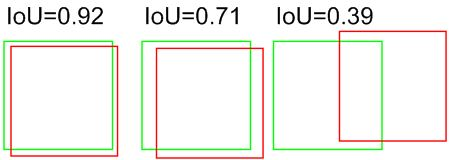
\includegraphics[scale=0.7]{figures/detector/iou.jpg}
    \caption[Caption for LOF]{IoU primjeri\footnotemark}
    \label{fig:iou}
\end{figure}
\footnotetext{https://www.interstellarengine.com/ai/Intersection-Over-Union.html}

\begin{figure}[H]
     \centering
     \foreach \i in {1,...,16} {
        \begin{subfigure}[b]{0.2\textwidth}
        \centering
        \includegraphics[width=\textwidth]{figures/input_examples/positive/\i.jpg}
        \end{subfigure}
        \pgfmathparse{Mod(\i,4)==0?1:0}
        \ifnum \pgfmathresult>0 \\[0.3cm] \else \hspace{0.3cm} \fi
     }
    \caption{Pozitivni primjeri ulaznih podataka}
    \label{fig:input_examples_positive}
\end{figure}

\begin{figure}[H]
     \centering
     \foreach \i in {1,...,16} {
        \begin{subfigure}[b]{0.2\textwidth}
        \centering
        \includegraphics[width=\textwidth]{figures/input_examples/negative/\i.jpg}
        \end{subfigure}
        \pgfmathparse{Mod(\i,4)==0?1:0}
        \ifnum \pgfmathresult>0 \\[0.3cm] \else \hspace{0.3cm} \fi
     }
    \caption{Negativni primjeri ulaznih podataka}
    \label{fig:input_examples_negative}
\end{figure}

\chapter{Prepoznavanje registarskih tablica}
Drugi korak, ujedno i posljednji, sustava za detekciju i prepoznavanje registarskih tablica je prepoznavanje istih. Na temelju pronađene registarske tablice potrebno je prvo segmentirati znakove, a zatim ih prepoznati. U literaturi se ovaj postupak naziva i optičko prepoznavanje znakova \engl{optical character recognition, OCR}. Postoji puno različitih pristupa problemu. U ovom radu pokušavamo prepoznati registarske tablice pa promatramo prepoznavanje štampanih znakova. Također, postoji i pristup prepoznavanja rukom pisanih znakova koji je nešto složeniji zbog svoje dinamičnosti jer, u velikoj većini slučajeva, različite osobe imaju različiti rukopis.

Prirodan tijek prepoznavanja registarskih tablica bio bi sljedeći: dobivenu sliku registarske tablice iz sustava za detekciju potrebno je obraditi tako da znakovi iste budu relativno lako odvojivi. Dakle, možda je potrebno poboljšati kontrast, napraviti binarizaciju, pronaći konture znakova tako da se promatra povezanost piksela istog intenziteta i sl. Jednom kada su znakovi pronađeni, iste je potrebno transformirati u neki prostor značajki koji naučeni klasifikator razumije. Već smo spomenuli neke kombinacije značajki i klasifikatora koje vrijede i ovdje. Najčešći pristup je izgraditi bazu podataka svih znakova te istom naučiti neku unaprijednu potpuno povezanu neuronsku mrežu koja na ulazu dobiva značajke konvolucijske neuronske mreže \citep{zemris}. No, što ako su registarske tablice malo rotirane? Što ako su u perspektivi? Što ako su dvoretčane? Što ako je neki znak malo prekriven zbog prljavštine ili zbog položaja kamere kao na slici \ref{fig:ce_gauss_tamniji}? Segmentacija znakova se drastično otežava zbog navedenih problema, a time i učenje samog klasifikatora jer je i bazu znakova potrebno izgraditi tako da prepoznaje rotirane znakove i sl.\ čime se uvelike otežava sam proces konstrukcije sustava.

Ispravljanje iskrivljenih \engl{skewed} registarskih tablica može se postići perspektivnom transformacijom \engl{perspective transformation} gdje se prvo na slici pronađe rotirani pravokutnik u kojem se registarske oznake nalaze, a zatim se isti transformira u 2-D ravninu. Problem se javlja kod pronalaska rotiranog pravokutnika. Postoji nekoliko pristupa kako se isto određuje, a u radu su promatrana dva. Prvi pristup bio je pronalazak linija pomoću Houghove transformacije, dok drugi pronalazak konveksne ljuske \engl{convex hull} registarske tablice pomoću koje se pokušava aproksimirati poligon s četiri vrha. Navedeni pristupi nisu pokazivali dovoljno dobre rezultate pa se od istih odustalo. Problem je što pristup radi na dvije slike, a na trećoj već ne itd\footnote{Možda navedeni pristupi i nisu toliko loši kada se jako dobro razumiju i razrade. U ovom radu to nije bio slučaj.}.

Kao rješenje svih navedenih problema, ili barem većine, su duboki modeli. Ideja je da se znakovi registarske tablice više ne pronalaze algoritmima računalnog vida \engl{computer vision}, već algoritmima dubokog učenja \engl{deep learning} upravo zbog robusnosti. Koncept je sljedeći: podijeli sliku registarske tablice na $n$ jednakih dijelova povlačeći vertikalne linije, a zatim svaki od tih dijelova predaj klasifikatoru s pamćenjem koji će znati odrediti predstavlja li predani ulaz dio nekog znaka ili dio pozadine. U literaturi se ovaj problem naziva problem označavanja slijeda \engl{sequence labeling}. Jedan od efikasnijih klasifikatora za ovakve probleme su povratne neuronske mreže \engl{recurrent neural network, RNN} koje se jednostavno uz dovoljan broj primjera mogu boriti s rotiranim znakovima, prekrivenim znakovima itd. Ukratko, mogu se boriti sa svim ranije navedenim problemima.

Sustavu za prepoznavanje registarskih oznaka ćemo pristupiti na isti način kao i sustavu za detekciju istih. Prvo ćemo dati kratak osvrt o povratnim neuronskim mrežama, a zatim ćemo dati opis modela sustava za prepoznavanje registarskih tablica, funkcije gubitka i prikazat ćemo izgled ulaznih podataka sustava, dok ćemo o optimizaciji pričati u poglavlju o rezultatima.

\section{Povratne neuronske mreže}
Povratne neuronske mreže primjer su neuronskih mreža koje obrađuju slijedne podatke \engl{sequential data}. Neki od područja primjena su strojno prevođenje \engl{machine translation}, označavanje vrste riječi \engl{part-of-speech tagging}, analiza sentimenta \engl{sentiment analysis} i dr. Za razliku od unaprijednih potpuno povezanih neuronskih mreža, na ulazu mogu dobivati sljedove različitih duljina a da pritom koriste iste parametre. Dakle, broj parametara povratne neuronske mreže ne ovisi o duljini ulaznog slijeda. Princip dijeljenja parametara je sličan kao i kod konvolucijskih neuronskih mreža, osim što konvolucije djeluje lokalno u ovisnosti o susjedstvu, dok svi parametri povratne neuronske mreže djeluju na svaki sljedeći podatak. To je moguće zbog toga što povratna neuronska mreža pored trenutnog stanja prati i svako prijašnje, odnosno može se reći da se prati cjelokupni kontekst dosad viđenih podataka.

Inspiracija za navedeno je dinamički sustav prikazan na slici \ref{fig:dynamic}. Sustav posjeduje neko stanje $h^{(t-1)}$ koje dovedenim ulazom $x^{(t)}$ ažurira pomoću neke funkcije $f$:
\begin{equation}
    h^{(t)} = f(h^{(t-1)},x^{(t)}).
\end{equation}
Funkcija $f$ neovisna je o koraku $t$ i kada se radi o jednostavnim povratnim neuronskim mrežama poput Elmanove, definirana je na sljedeći način \citep{duboko}:
\begin{equation}
    h^{(t)} = g(W_{hh}h^{(t-1)} + W_{xh}x^{(t)} + b_h),
    \label{eq:hidden_state}
\end{equation}
gdje $g$ predstavlja funkciju nelinearnosti (\textit{npr}.\ sigmoida, tangens hiperbolni, zglobnica), $W_{hh}$ i $W_{xh}$ matrice parametara, a $b_h$ vektor pristranosti. Dakle, stanje $h^{(t)}$ sadrži reprezentaciju, tj.\ kontekst dosad viđenih podataka. Dimenzionalnosti stanja i ulaza ne moraju biti jednaki i često nisu, a za njihovu kompatibilnost su zaslužne matrice parametara. Stanje $h^{(t)}$ često zna sadržavati i neke nebitne informacije o konkretnim podacima koje ne pospješuju generalizaciju. Kako bi se navedeno riješilo, uveden je još izlazni sloj koji je definiran na sljedeći način:
\begin{equation}
    o^{(t)} = W_{hy}h^{(t)} + b_o,
    \label{eq:output_state}
\end{equation}
gdje $W_{hy}$ predstavlja matricu parametara i projekciju stanja na izlaz, a $o^{(t)}$ \textit{logit} vrijednost izlaza koja se dalje koristi za funkciju gubitka. Time je jednostavna povratna neuronska mreža definirana.

\begin{figure}
    \centering
    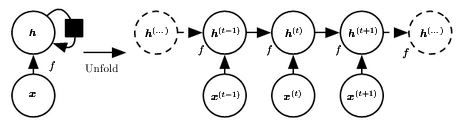
\includegraphics[scale=0.7]{figures/recognizer/dynamic.jpg}
    \caption[Caption for LOF]{Razmatanje dinamičkog sustava\footnotemark}
    \label{fig:dynamic}
\end{figure}
\footnotetext{Preuzeto iz \citep{Goodfellow-et-al-2016}.}

Na slici \ref{fig:rnn} nalazi se primjer vremenski razmotane povratne neuronske mreže. Slike je preuzeta iz \citep{Goodfellow-et-al-2016} i potrebno je objasniti neke razlike: $U=W_{xh}, W=W_{hh}$ i $V=W_{hy}$. Oznake u formulama \ref{eq:hidden_state} i \ref{eq:output_state} su u skladu s \citep{duboko} jer su intuitivnije od navedenih slova $U, W$ i $V$, ali slika je jako zgodna te je zbog toga uzeta. Na slici postoje još dvije oznake $L$ i $y$. $L^{(t)}$ predstavlja gubitak između $o^{(t)}$ i $y^{(t)}$, dok $y^{(t)}$ stvarnu oznaku u trenutku $t$.

Ovako definirana arhitektura povratne neuronske mreže u kontekstu gradi reprezentaciju na temelju svih vremenskih trenutaka do trenutnog. To u nekim primjenama nije dovoljno jer želimo moći vidjeti i jedan dio konteksta koji dolazi u budućnosti kako bi točnije dali odluku o rezultatu. Najbolji primjer je strojno prevođenje gdje je potreban kontekst prije trenutne riječi, ali i kontekst nakon iste jer jedna riječ može imati puno značenja. Problem se rješava tako da se doda još jedna povratna neuronska mreža u suprotnom smjeru. To znači da jedna neuronska mreža ulaz dobiva s lijeva nadesno, dok druga obratno. U literaturi se ovakva neuronska mreža naziva dvosmjerna povratna neuronska mreža \engl{bidirectional RNN, BiRNN} i primjer jedne takve neuronske mreže nalazi se na slici \ref{fig:bi-rnn}. $g^{(t)}$ predstavlja sloj u kojem se računa novo stanje $h^{(t)}$ kao konkatenacija stanja obje mreže: $h^{(t)} = [\overrightarrow{h}^{(t)}, \overleftarrow{h}^{(t)}]$.

\begin{figure}[H]
    \centering
    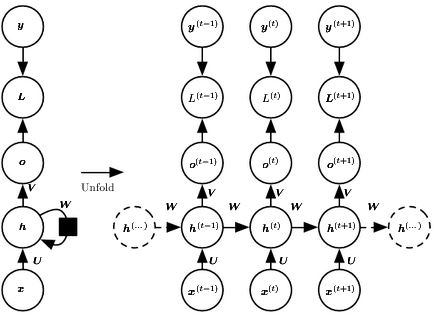
\includegraphics[scale=0.7]{figures/recognizer/rnn.jpg}
    \caption{Razmotani RNN}
    \label{fig:rnn}
\end{figure}

\begin{figure}[H]
    \centering
    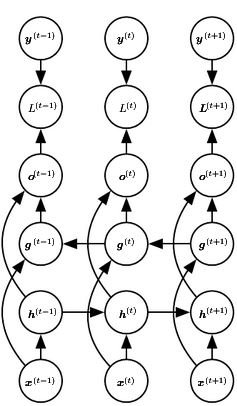
\includegraphics[scale=0.7]{figures/recognizer/bi-rnn.jpg}
    \caption[Caption for LOF]{Razmotani BiRNN\footnotemark}
    \label{fig:bi-rnn}
\end{figure}
\footnotetext{Preuzeto iz \citep{Goodfellow-et-al-2016}.}

Povratne neuronske mreže se uče algoritmom propagacije pogreške unatrag kroz vrijeme \engl{backpropagation through time algorithm, BPTT} koji je konceptualno vrlo sličan originalnom algoritmu korištenom pri učenju unaprijedne neuronske mreže, osim što se u obzir uzimaju vremenski koraci i različiti smjerovi putovanja gradijenata kod dvosmjernih povratnih neuronskih mreža. Istim se ne bavimo u ovom radu, a više detalja se može pronaći u \citep{duboko} i \citep{Goodfellow-et-al-2016}. 

Dosad smo promatrali samo jednoslojne povratne mreže, no iste se mogu konstruirati s više slojeva i to najčešće od 4 do 8. Stanje jednog sloja glumi ulaz drugom sloju itd.\ Navedeni RNN model pati od problema iščezavajućeg i eksplodirajućeg gradijenta. Naime, parametri $W_{hh}$ i $W_{xh}$ služe za filtriranje nepotrebnih informacija, pamćenje dosad viđenih ulaza, projekciju itd. Njihovim opetovanim množenjem pri propagaciji pogreške sustav postaje jako nestabilan. Očigledno je da navedeni parametri imaju preveliku odgovornost. Kako bi se problem riješio, kreirana je nova povratna mreža imena povratna neuronska mreža s dugoročnom memorijom \engl{long short-term memory, LSTM}.

LSTM uvodi tzv.\ propusnicu zaboravljanja \engl{forget gate} i propusnicu ulaza \engl{input gate}. Ideja propusnice zaboravljanja je izbaciti dio informacija iz prošlog stanja jer je očigledno da se vremenom isto može zasititi nebitnim stvarima. Ideja propusnice ulaza je propustiti samo podskup informacija iz ulaza jer neke nisu od koristi. Formule za navedene konstrukte su identične formuli \ref{eq:hidden_state} uz sigmoidu kao funkciju nelinearnosti, osim što svaki od navedenih ima svoj skup parametara (\textit{i.e}.\ $W_{fhh}, W_{ihh}$ itd.). Također, $h^{(t)}$ se prenamjenjuje samo za skrivenu reprezentaciju, dok se za pamćenje dosadašnjih informacija uvodi novi vektor $c^{(t)}$. Time se dvostruka zadaća stanja RNN mreže razdvojila. Kako bi se izbjeglo množenje pri propagaciji pogreške unatrag, uveden je još jedan pomoćni vektor $\hat{c}^{(t)}$ u kojem držimo vrijednost kojom ažuriramo stanje $c^{(t)}$. Stanje $c^{(t)}$ računa se onda na sljedeći način:
\begin{equation}
    c^{(t)} = f^{(t)} \odot c^{(t-1)} + i^{(t)} \odot \hat{c}^{(t)},
\end{equation}
gdje je $\odot$ Hadamardov umnožak\footnote{Množenje vektora po elementima.}, a $\hat{c}^{(t)}$ je isto definiran formulom \ref{eq:hidden_state} uz tangens hiperbolni kao funkciju nelinearnosti i svojim skupom parametara. Propusnica izlaza \engl{output gate} $o^{(t)}$ se također računa kao i ranije navedene propusnice uz naravno svoj skup parametara. Na kraju, skrivena reprezentacija
$h^{(t)}$ računa se na sljedeći način:
\begin{equation}
    h^{(t)} = o^{(t)} \odot \tanh(c^{(t)}).
\end{equation}
LSTM očigledno ima 4 puta više parametara nego RNN, ali se dvojaka uloga stanja druge razbila čime se olakšava generalizacija prilikom učenja i izbjegavaju se problemi oko gradijenata. Na slici \ref{fig:lstm} nalazi se primjer LSTM čelije.

\begin{figure}[H]
    \centering
    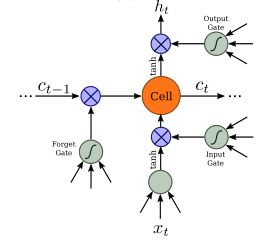
\includegraphics[scale=0.7]{figures/recognizer/lstm.jpg}
    \caption[Caption for LOF]{LSTM primjer\footnotemark}
    \label{fig:lstm}
\end{figure}
\footnotetext{Preuzeto iz \citep{crnn-paper}.}

Ovdje smo se dotaknuli samo najopćenitijih stvari oko povratnih neuronskih mreža. Puno više detalja se može pronaći u \citep{duboko}, \citep{Goodfellow-et-al-2016} i \citep{rnn-paper}.

\section{Model sustava za prepoznavanje}
Model sustava za prepoznavanje baziran je na radu \citep{crnn-paper}. Arhitektura konvolucijske neuronske mreže za izlučivanje značajki je ista kao i kod sustava za detekciju, a arhitektura klasifikatora znakova nalazi se u tablici \ref{tab:recognizer}. Svi tipovi slojeva su već opisani jedino ćemo spomenuti veličinu skrivene reprezentacije povratne neuronske mreže kao i broj ulaznih, odnosno izlaznih neurona konačnog sloja \textit{Linear}. \textit{\#hidden units} predstavlja veličinu skrivene reprezentacije i ona je ovdje postavljena na 64, dok je u izvornom radu postavljena na 128. Broj ulaza sloja \textit{Linear} iznosi $64\cdot2 = 128$, gdje 64 dolazi od veličine skrivene reprezentacije, a 2 zbog toga što se radi o dvosmjernoj povratnoj neuronskoj mreži. Broj izlaza iznosi 37 jer postoji 36 mogućih znakova (\textit{i.e}.\ 10 znamenki i 26 slova engleske abecede) i još jedan koji predstavlja pozadinu. Izlazi ili \textit{logiti} sloja \textit{Linear} na kraju prolaze kroz funkciju nelinearnosti softmax kako bi se generirala vjerojatnosna distribucija znakova sekvence.

Dakle, prvo se pomoću konvolucijske neuronske mreže generiraju značajke za ulaznu sliku, a zatim se iste provlače kroz klasifikator sastavljen od povratne neuronske mreže. Ovakav pristup nazvan je konvolucijska povratna neuronska mreža \engl{convolutional recurrent neural network, C-RNN}. S obzirom na to da oblik generiranih značajki ne odgovara željenom ulazu povratne neuronske mreže, potrebno je napraviti malu projekciju na sljedeći način: širina konačne slike predstavlja duljinu ulazne sekvence, a visina konačne slike $\times$ broj izlaznih mapa značajki predstavlja broj značajki znaka sekvence. Konkretno u našem slučaju: dimenzionalnost značajki konvolucijske neuronske mreže je $128\times1\times24$. To znači da je duljina ulazne sekvence 24 i da je svaki element iste vektor veličine 128. Valja napomenuti kako je duljina sekvence ovdje simbolično uvijek 24 zbog toga što je ulazna slika uvijek skalirana na veličinu $32\times100$. U izvornom radu \citep{crnn-paper} se navedeno skaliranje koristi zbog brzine učenja i da visina uvijek dosegne jedan piksel. Stoga, ako je širina slike proizvoljne širine, svejedno će algoritam uspješno raditi jer povratne neuronske mreže mogu obraditi proizvoljnu duljinu sekvenci. Na slici \ref{fig:crnn-features} je upravo navedeni postupak i prikazan.

\bigskip

\begin{table}[H]
    \centering
    \begin{tabular}{|c|c|}
        \hline
        Tip sloja & Konfiguracija \\
        \hline \hline
        BiLSTM & \#hidden units:64\\
        \hline
        Dropout & p \\
        \hline
        BiLSTM & \#hidden units:64 \\
        \hline
        Linear & in:64$\cdot$2, out:37 \\
        \hline
        Softmax & - \\
        \hline
    \end{tabular}
    \caption{Konfiguracija modela za klasifikaciju}
    \label{tab:recognizer}
\end{table}

\begin{figure}[H]
    \centering
    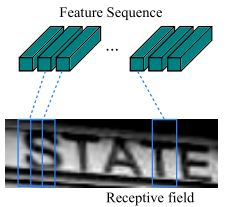
\includegraphics[scale=0.7]{figures/recognizer/crnn-features.jpg}
    \caption[Caption for LOF]{Prikaz značajki kao sekvenca znakova\footnotemark}
    \label{fig:crnn-features}
\end{figure}
\footnotetext{Preuzeto iz \citep{crnn-paper}.}

\section{Gubitak vremenski povezane klasifikacije}
Problem s kojim se susrećemo prilikom prepoznavanja registarskih tablica je kako točno klasificirati sekvencu ako ne znamo koji dijelovi sekvence odgovaraju pozadini, a koji nekome od znakova. Ovo se vrlo lako može označiti ručno tako da svaki dio sekvence ima svoju oznaku. Problem se onda pretvara u jednostavnu višerazrednu klasifikaciju gdje se može koristiti gubitak unakrsne entropije. No ručno označavanje je vremenski zahtjevno i definitivno nije opcija. Vremenski povezana klasifikacija \engl{connectionist temporal classification, CTC} rješava navedeni problem tako da nije potrebno znati oznake svih dijelova sekvenci, već konačni ishod, a sam algoritam će se pobrinuti da se to ostvari.

Prikažimo vremensku klasifikaciju formalno. Neka je $S$ skup podataka za učenje generiranih iz distribucije $D_{X \times Z}$, gdje $\mathbf{X} = (\mathbb{R}^m)^*$ predstavlja skup svih ulaznih sekvenci m-dimenzionalnih vektora, a $\mathbf{Z} = L^*$ predstavlja skup svih sekvenci konačnog skupa željenih znakova $L$. U našem slučaju, željeni znakovi su znamenke i velika slova engleske abecede. Svaki primjer skupa $S$ je uređeni par sekvenci $(\pmb{\mathbf{x}}, \pmb{\mathbf{z}})$, gdje $\pmb{\mathbf{x}} = (x_1, x_2, \dots, x_T)$, $\pmb{\mathbf{z}} = (z_1, z_2, \dots, z_U)$ i $U \leq T$. Pomoću skupa $S$ potrebno je naučiti klasifikator $h: \mathbf{X} \mapsto \mathbf{Z}$ koji će biti u stanju klasificirati neviđene sekvence. Kako bi to bilo ostvarivo, potrebno je konstruirati funkciju gubitka pa krenimo.

Neka je definirana povratna neuronska mreža $N$ s $m$ ulaza, $n$ izlaza i vektorom težina $w$. Tada vrijedi $N_w : (\mathbb{R}^m)^T \mapsto (\mathbb{R}^n)^T$. Neka je $\pmb{\mathbf{y}} = N_w(\pmb{\mathbf{x}})$ sekvenca izlaza povratne neuronske mreže. Neka je $y_k^t$ aktivacija neurona $k$ u trenutku $t$. Tada se $y_k^t$ može interpretirati kao vjerojatnost pojave k-tog znaka u trenutku $t$. Ovo je moguće interpretirati na ovaj način jer \textit{logiti} klasifikatora prolaze kroz funkciju nelinearnosti softmax koja mapira sve ulazne vrijednosti u vjerojatnosne čija krajnja suma uvijek mora biti 1. Kako bi uključili klasifikaciju pozadine, potrebno je nadodati još jedan znak u skup $L$: $L^{'} = L \cup \{blank\}$. Iz navedenog se može definirati sljedeća vjerojatnost:
\begin{equation}
    p(\pi | \pmb{\mathbf{x}}) = \prod_{t=1}^{T}y_{\pi_t}^t, \forall \pi \in {L^{'}}^T.
    \label{eq:pi_prob}
\end{equation}
Sekvence sastavljene od elemenata skupa ${L^{'}}^T$ se u izvornom radu \citep{ctc-paper} nazivaju putanje \engl{paths} i označavaju se s $\pi$. Formula je zapisana kao produkt vjerojatnosti jer se implicitno pretpostavlja da su izlazi povratne neuronske mreže u različitim vremenima nezavisni i identično distribuirani \engl{independently and indentically distributed, IID}. S obzirom na to da želimo dobiti sekvencu duljine $\leq T$, a duljina sekvence $\pi$ je $T$, potrebno je konstruirati funkciju mapiranja $B : {L^{'}}^T \mapsto L^{\leq T}$. Funkcija $B$ je tzv.\ \textit{many-to-one} funkcija koja mapira više različitih ulaza u isti izlaz i definirana je na sljedeći način:
\begin{itemize}
    \item makni sve \textit{blank} znakove iz sekvence,
    \item spoji sve ponavljajuće znakove.
\end{itemize}
Npr.\ $B(A-AB-) = B(-AA--ABB) = AAB$. Sada napokon možemo definirati vjerojatnost izlazne sekvence, odnosno funkciju gubitka, na temelju ulazne sekvence kao sumu vjerojatnosti svih putanja koje funkcija $B$ mapira u željenu sekvencu:
\begin{equation}
    p(\pmb{\mathbf{l}} | \pmb{\mathbf{x}}) = \sum_{\pi : B(\pi) = \pmb{\mathbf{l}}}p(\pi|\pmb{\mathbf{x}}).
    \label{eq:l_seq}
\end{equation}
Klasifikator vremenski povezane klasifikacije je onda definiran na sljedeći način:
\begin{equation}
    h(\pmb{\mathbf{x}}) = \argmax_{\pmb{\mathbf{l}} \in L^{\leq T}}p(\pmb{\mathbf{l}} | \pmb{\mathbf{x}}).
\end{equation}
Pronalazak sekvence $\pmb{\mathbf{l}}$ se u litaraturi \citep{ctc-paper} naziva i problemom dekodiranja \engl{decoding}. Očigledno je da je izračun formule \ref{eq:l_seq} vremenski izrazito zahtjevan jer broj putanja $\pi$ može biti jako velik. Kako bi se problem izbjegao, postoje dva poznata pristupa. U prvom pristupu, ujedno i korištenom u ovom radu, se pohlepno dekodiraju uvijek najvjerojatniji znakovi sekvence \engl{best path decoding} u trenutku $t$:
\begin{equation}
    \pi^* = \argmax_{\pi \in N^t}p(\pi | \pmb{\mathbf{x}}).
\end{equation}
Drugi pristup koristi tzv.\ pretraživanje zrakama \engl{beam search} i nije korišten u ovom radu, a više o istom može se pronaći u \citep{ctc-paper}.

Konačno, možemo definirati i funkciju pogreške koju je potrebno minimizirati:
\begin{equation}
    E = - \sum_{(\pmb{\mathbf{x}}, \pmb{\mathbf{z}}) \in S} \ln p(\pmb{\mathbf{z}}|\pmb{\mathbf{x}}).
\end{equation}

Sam pronalazak putanji $\pi$ i izračun svih uvjetnih vjerojatnosti \ref{eq:l_seq} i gradijenata tijekom učenja izvodi se algoritmom naprijed nazad \engl{forward-backward algorithm} koji je primjer dinamičkog programiranja. U ovom radu ne ulazimo u detalje izvoda izračuna, a više se može pronaći u \citep{ctc-paper} i \citep{crnn-paper}. 

\section{Primjeri ulaznih podataka}
Izgled i postupak generiranja primjera za učenje je gotovo pa identičan postupku opisanom kod sustava za detekciju. Glavna razlika je što se sada uvijek generiraju primjeri koji sadrže registarsku tablicu jer ostali negativni primjeri ne nose nikakve potrebne informacije za sustav.


\chapter{Rezultati}
U sklopu ovog rada, pored teorijske podloge, implementiran je prototip sustava za prepoznavanje registarskih tablica. Sustav je implementiran pomoću programskog jezika \textit{Python} zbog svoje jednostavnosti i velikog broja gotovih modula. Za obradu slika i algoritam selektivno pretraživanje korišten je modul \textit{OpenCV}, za implementaciju dubokih modela korišten je modul \textit{Pytorch Lightning}, dok je za izradu grafičkog sučelja sustava korišten modul \textit{Tkinter}. Zbog nedostatka kvalitetne grafičke kartice, duboki modeli trenirani su pomoću \textit{Google Colab} platforme koja nudi virtualan stroj s jednom grafičkom karticom.

\section{Opis baze podataka}
Baza podataka nad kojom je sustav izgrađen preuzeta je iz \citep{zemris}. Sastoji se od ukupno 509 slika automobila dimenzija $640 \times 480$\footnote{Ovdje je zapis obratan u odnosu na onaj kod opisa konvolucijskog modela pa prva vrijednost predstavlja širinu, a druga visinu slike.}. Par slika je slikano sprijeda, no uglavnom su slikani stražnji dijelovi. Uvjeti slikanja su raznoliki pa tako postoje slike po danu, po noći, pod sjenom, u perspektivi itd. Također, iako su u manjini, postoje primjeri dvoretčanih tablica i tablica sa svijetlim slovima.

U sklopu ovog rada, implementiran i je pomoćni sustav koji služi za označavanje \engl{annotation} pozicija graničnih okvira registarskih tablica kao i sadržaj istih pa je tako cijela baza ručno označena. Oznake su prvo korištene za generiranje podataka za učenje kao što je i opisano u radu. Kao granica mjere IoU za pozitivne primjere generirane selektivnim pretraživanjem, postavljena je vrijednost $0.7$, dok je za negativne $0.05$. Također, kako broj negativnih primjera ne bi bio puno veći od pozitivnih, gornja granica za generiranje negativnih primjera je 15, dok je za pozitivne 20. Broj negativnih primjera će uvijek biti 15, dok broj pozitivnih varira ovisno o tome koliko dobro selektivno pretraživanje uspije pronaći granične okvire registarske tablice. Ovo naravno vrijedi za sustav za detekciju, dok se za sustav za prepoznavanje generiraju samo primjeri koji sadrže registarske tablice, dakle, samo pozitivni primjeri iz perspektive prvog sustava. Sve navedeno, naravno, vrijedi za jednu sliku, što znači da se postupak provodi nad svakom slikom. U tablici \ref{tab:data} prikazana je veličina skupa za učenje i validaciju oba sustava. Omjer skupa za učenje i skupa za validaciju je $80:20$.

\begin{table}[H]
    \centering
    \begin{tabular}{|c|c|c|}
        \hline
        Skup & Sustav za detekciju & Sustav za prepoznavanje \\
        \hline \hline
        Učenje & 13474 & 11240 \\
        \hline
        Validacija & 3440 & 2570 \\
        \hline
    \end{tabular}
    \caption{Broj primjera za učenje i validaciju sustava}
    \label{tab:data}
\end{table}

\section{Optimizacija}
Optimizacijski algoritam korišten za učenje oba modela je Adam i to uz regularizaciju\footnote{U poznatim programskim bibliotekama se također naziva i AdamW od \textit{Adam with weight decay}.}. Navedeni algoritam je korišten jer se pokazuje kao najbolji za implementaciju prototipnog sustava s obzirom na to da ga nije potrebno previše prilagođavati zbog toga što sam vodi brigu o iznosu stope učenja praćenjem gradijenata i kvadrata gradijenata uz eksponencijalno zaboravljanje. Detalji se mogu pronaći u \citep{adamw-paper}. Parametri algoritma korišteni za treniranje modela ovog rada su prikazani u tablici \ref{tab:adamw}.

\begin{table}[H]
    \centering
    \begin{tabular}{|c|c|}
        \hline
        Parametar & Vrijednost \\
        \hline \hline
        $\eta$ & 1e-3 \\
        \hline
        $(\beta_1,\beta_2)$ & {(0.9, 0.999)} \\
        \hline
        $\lambda$\footnotemark & 1e-4 \\
        \hline
    \end{tabular}
    \caption{Parametri algoritma Adam}
    \label{tab:adamw}
\end{table}
\footnotetext{Regularizacijski faktor.}

Kako bi se dodatno osvježavao iznos stope učenja, korištene je planer stop učenja \engl{learning rate scheduler} koji smanjuje stopu učenja za neki faktor ako se promatrana mjera određeni broj epoha nije poboljšala \engl{reduce learning rate on plateau}. Navedeni planer je koristan ako je u jednom trenutku potrebno raditi puno manje korake u optimizaciji jer smo bliže nekom optimumu. Istovremeno može biti i loš ako se ne radi o globalnom optimumu jer smanjivanjem stope učenja ćemo se teško iskopati iz lokalnog optimuma, no u ovom radu nije bilo problema s time. U tablici \ref{tab:scheduler} prikazani su parametri oba sustava gdje \textit{patience} predstavlja broj epoha bez promjene promatrane mjere na bolje, a \textit{min} $\eta$ predstavlja donju ogradu stope učenja. Dakle, ako se mjera ne poboljšava, stopa učenja se smanjuje za deset puta. \textit{patience} vrijednosti se razlikuju za oba sustava jer se radi o drugačijim problemima i broj ukupnih epoha učenja će biti različit, što ćemo i vidjeti u nastavku.

\begin{table}[H]
    \centering
    \begin{tabular}{|c|c|c|}
        \hline
        Parametar & Sustav za detekciju & Sustav za prepoznavanje \\
        \hline \hline
        factor & 0.1 & 0.1 \\
        \hline
        patience & 8 & 10 \\
        \hline
        min $\eta$ & 1e-7 & 1e-7 \\
        \hline
    \end{tabular}
    \caption{Parametri planera stope učenja}
    \label{tab:scheduler}
\end{table}

\section{Modeli}
U tablici \ref{tab:models} se nalazi broj parametara i memorijsko zauzeće pojedinog modela. Model za detekciju ima skoro sedam puta više parametara nego model za prepoznavanje. To je upravo zbog toga što se kod prvog kao klasifikator koristi unaprijedna potpuno povezana neuronska mreža, dok se kod drugog koristi povratna neuronska mreža koja dijeli parametre kroz vrijeme te time znatno štedi memorijski prostor.
\begin{table}[H]
    \centering
    \begin{tabular}{|c|c|c|}
        \hline
         & Sustav za detekciju & Sustav za prepoznavanje \\
        \hline \hline
        Broj parametara & 3.8 M & 551 K \\
        \hline
        Zauzeće u MB & 15.028 & 2.204 \\
        \hline
    \end{tabular}
    \caption{Broj parametara i memorijsko zauzeće modela}
    \label{tab:models}
\end{table}

Sukladno tomu su postavljene i vjerojatnosti sloja \textit{Dropout} u tablici \ref{tab:dropout}. Model za detekciju ima veću vjerojatnost zbog većeg broja parametara kako bi se ublažila prenaučenost.
\begin{table}[H]
    \centering
    \begin{tabular}{|c|c|}
        \hline
        Sustav za detekciju & Sustav za prepoznavanje \\
        \hline \hline
        0.5 & 0.3 \\
        \hline
    \end{tabular}
    \caption{Vjerojatnost $p$ sloja \textit{Dropout}}
    \label{tab:dropout}
\end{table}
Svi parametri slojeva \textit{Linear} i \textit{Convolution} inicijalizirani su uniformnom verzijom Kaiming inicijalizacije, dok su parametri sloja \textit{LSTM} inicijalizirani uniformno iz intervala $[-\frac{1}{\sqrt{\text{\#hidden units}}}, \frac{1}{\sqrt{\text{\#hidden units}}}]$.

\section{Rezultati učenja}
Parametri samog procesa učenja nalaze se u tablici \ref{tab:train}. Broj epoha za sustav za prepoznavanje je nešto veći jer se pokazalo kako modelu za prepoznavanje treba nešto više vremena za učenje uz navedene tehnike optimizacije.

\begin{table}[H]
    \centering
    \begin{tabular}{|c|c|c|}
        \hline
        Parametar & Sustav za detekciju & Sustav za prepoznavanje \\
        \hline \hline
        Broj epoha & 50 & 100 \\
        \hline
        Veličina minigrupe & 128 & 128 \\
        \hline
    \end{tabular}
    \caption{Parametri procesa učenja}
    \label{tab:train}
\end{table}

Rezultati učenja i kretanja vrijednosti gubitaka prikazani su na slikama \ref{fig:loss_detector} i \ref{fig:loss_recognizer}. Očigledno su oba modela prenaučena. To se vidi po grafovima, ali vidjet će se i u prikazu točnosti samog sustava na kraju. Glavni problem je mala baza podataka i velika sličnost između skupa za učenje i validaciju s obzirom na to da su generirani na isti način pa se neki primjeri skoro pa identično ponavljaju u oba skupa. Kako bi se problem donekle smanjio, uvedeno je klasično uvećanje podataka \engl{data augmentation} tako što su primjeri za učenje prvo s vjerojatnosti 0.5 stavljeni u perspektivu, a zatim rotirani za slučajno izabrani kut iz $[-10^\circ, 10^\circ]$. Na slici \ref{fig:augmentation} su prikazani neki od primjera gdje prva slika predstavlja originalnu sliku, a ostale tri su uvećane navedenim pristupom.

\bigskip

\begin{figure}[H]
    \centering
    \begin{subfigure}[b]{0.2\textwidth}
        \centering
        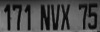
\includegraphics[width=\textwidth]{figures/augmentation/0.jpg}
    \end{subfigure}
    \hspace{0.1cm}
    \begin{subfigure}[b]{0.2\textwidth}
        \centering
        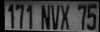
\includegraphics[width=\textwidth]{figures/augmentation/1.jpg}
    \end{subfigure}
    \hspace{0.1cm}
    \begin{subfigure}[b]{0.2\textwidth}
        \centering
        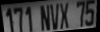
\includegraphics[width=\textwidth]{figures/augmentation/2.jpg}
    \end{subfigure}
    \hspace{0.1cm}
    \begin{subfigure}[b]{0.2\textwidth}
        \centering
        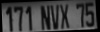
\includegraphics[width=\textwidth]{figures/augmentation/3.jpg}
    \end{subfigure}
    \caption{Primjeri uvećanja podataka}
    \label{fig:augmentation}
\end{figure}

\begin{figure}[H]
     \centering
     \begin{subfigure}[b]{0.4\textwidth}
         \centering
         \includegraphics[width=\textwidth]{figures/results/detector_train.jpg}
         \caption{Gubitak učenja}
     \end{subfigure}
     \hspace{0.5cm}
     \begin{subfigure}[b]{0.4\textwidth}
         \centering
         \includegraphics[width=\textwidth]{figures/results/detector_val.jpg}
         \caption{Gubitak validacije}
     \end{subfigure}
    \caption{Prikaz gubitaka modela za detekciju}
    \label{fig:loss_detector}
\end{figure}

\begin{figure}[H]
     \centering
     \begin{subfigure}[b]{0.4\textwidth}
         \centering
         \includegraphics[width=\textwidth]{figures/results/recognizer_train.jpg}
         \caption{Gubitak učenja}
     \end{subfigure}
     \hspace{0.5cm}
     \begin{subfigure}[b]{0.4\textwidth}
         \centering
         \includegraphics[width=\textwidth]{figures/results/recognizer_val.jpg}
         \caption{Gubitak validacije}
     \end{subfigure}
    \caption{Prikaz gubitaka modela za prepoznavanje}
    \label{fig:loss_recognizer}
\end{figure}

\section{Prikaz sustava i krajnjih rezultata}
Na slici \ref{fig:program} prikazano je grafičko sučelje prototipa sustava za prepoznavanje registarskih tablica. Ako se registarska tablica pronađe, onda se to područje zaokruži crvenim pravokutnikom i iznad se napiše prepoznati sadržaj. Postoje i slučajevi u kojima sustav za detekciju ne uspije pronaći registarsku tablicu. Tada se to dojavi korisniku primjerenom porukom.
\begin{figure}[H]
    \centering
    \includegraphics[scale=0.6]{figures/results/gui.jpg}
    \caption{Grafičko sučelje sustava}
    \label{fig:program}
\end{figure}
Testiranje sustava izvedeno je na računalu s procesorom \textit{AMD Ryzen 5 3600} koji u sebi ima šest jezgara. Vremensko izvođenje jednog prepoznavanja prikazano slikom \ref{fig:program} traje oko tri sekunde, gdje selektivno pretraživanje uzme oko 90\% ukupnog vremena. Nakon što selektivno pretraživanje pronađe potencijalne objekte, većina njih se i odbacuje jer ne zadovoljavaju neke od specifikacija poput validnog raspona širine i visine graničnog okvira kao i raspon njihovog omjera. Sve navedene mjere su statistički pronađene nad bazom podataka, što znači da ako slika sadrži registarsku tablicu koja ne zadovoljava određene širine, visine i omjere, neće se uzeti u obzir. To je potencijalni problem navedenog sustava kao i samo selektivno pretraživanje jer izrazito usporava isti.

Mjere korištene za promatranje uspješnosti sustava su sljedeće:
\begin{itemize}
    \item točnost detekcije \engl{detection accuracy},
    \item točnost prepoznavanja \engl{recognition accuracy},
    \item srednja vrijednost mjere IoU \engl{mean IoU},
    \item stopa pogrešno prepoznatih znakova \engl{character error rate} i
    \item stopa prepoznavanja netočnih duljina \engl{incorrect length}.
\end{itemize}
Točnost se računa na sljedeći način pomoću indikatorske funkcije:
\begin{equation}
    Accuracy = \frac{1}{N}\sum_{i=1}^{N}1(y_i=\hat{y_i}),
\end{equation}
gdje $y_i$ predstavlja željenu vrijednost, a $\hat{y_i}$ stvarnu. Za prepoznavanje tražimo potpunu jednakost, dok kod detekcije, ako je mjera IoU $\geq$ 0.5, onda ulazi u skup točnih primjera.
Srednja vrijednost mjere IoU računa se na sljedeći način:
\begin{equation}
    IoU_{mean} = \frac{1}{N}\sum_{i=1}^{N}\text{IoU}(t_i, r_i),
\end{equation}
gdje $t_i$ predstavlja željeni granični okvir, a $r_i$ granični okvir pronađen sustavom za detekciju.
Stopa pogrešno prepoznatih znakova računa se na sljedeći način:
\begin{equation}
    Character Error Rate = \frac{S+D+I}{N},
\end{equation}
gdje $S$ označava broj izmjena \engl{substitutions} znakova, $D$ broj brisanja \engl{deletions} znakova, $I$ broj umetanja \engl{insertions} novih znakova, a $N$ ukupan broj znakova. Što je navedena mjera manja, to je sustav točniji. U literaturi je navedeni princip poznatiji kao Levenshteinova udaljenost \engl{Levenshtein distance}.
Stopa prepoznavanja netočnih duljina račun se na sljedeći način pomoću indikatorske funkcije:
\begin{equation}
    Incorrect Length = \frac{1}{N}\sum_{i=1}^{N}1(\text{length}(y_i)\ne\text{length}(\hat{y_i})).
\end{equation}

Prisjetimo se da selektivno pretraživanje nedeterminizmom grupira izlaze, što zapravo malo šteti sustavu za detekciju zbog toga jer sustav ne gleda npr.\ najboljih $k$ predikcija pa nad njima dodatno radi predikcije, već uvijek uzme prvu najbolju predikciju koja ne mora nužno biti najbolja, no iz perspektive modela ona ispada najboljom. To je također jedna od mana promatranog sustava. Na slici \ref{fig:ss-randomness} je ta pojava i prikazana. U prvom pokretanju sustava dobije se netočno prepoznavanje, dok se u sljedećem pokretanju dobije točno prepoznavanje.

\begin{figure}[H]
     \centering
     \begin{subfigure}[b]{0.4\textwidth}
         \centering
         \includegraphics[width=\textwidth]{figures/results/nondeterministic/incorrect_first.jpg}
         \caption{Netočno prepoznavanje}
     \end{subfigure}
     \hspace{0.5cm}
     \begin{subfigure}[b]{0.4\textwidth}
         \centering
         \includegraphics[width=\textwidth]{figures/results/nondeterministic/correct_second.jpg}
         \caption{Točno prepoznavanje}
     \end{subfigure}
    \caption{Primjer nedeterminizma sustava}
    \label{fig:ss-randomness}
\end{figure}

Kako bi se navedena pojava uzela u obzir prilikom testiranja sustava, sustav je pokrenut tri puta nad istom slikom gdje se na kraju uzima rezultat s najboljom mjerom IoU. U tablici \ref{tab:results} su prikazani rezultati testiranja originalne baze nad kojom je sustav učen, dakle nad svih 509 slika, i rezultati testiranja testne baze koja se sastoji od 10 slika. Ono što se može vidjeti je da sustav za detekciju radi iznimno dobro s obzirom na veličinu baze podataka nad kojom je učen. Sustav za prepoznavanje radi nešto lošije na glavnoj bazi podataka, dok nad testnom bazom radi izrazito loše, ali to je bilo i za očekivati. Jednostavno sustav nije vidio dovoljan broj primjera i kombinacija znakova da može dobro generalizirati. Previše se naučio nad glavnom bazom, što smo vidjeli i po grafovima kretanja gubitaka.

\begin{table}[H]
    \centering
    \begin{tabular}{|c|c|c|}
        \hline
        Mjera & Glavna baza & Testna baza \\
        \hline \hline
        Detection Accuracy & 0.97642 & 1.00000 \\
        \hline
        Recognition Accuracy & 0.92927 & 0.30000 \\
        \hline
        Mean IoU & 0.81306 & 0.74750 \\
        \hline
        Character Error Rate & 0.03187 & 0.17500 \\
        \hline
        Incorrect Length & 0.05501 & 0.30000 \\
        \hline
    \end{tabular}
    \caption{Rezultati sustava}
    \label{tab:results}
\end{table}

Na slikama \ref{fig:testdb_results}, \ref{fig:failed_detection} i \ref{fig:failed_recognition} prikazani su neki od probranih rezultata.

\begin{figure}[H]
     \centering
     \begin{subfigure}[b]{0.4\textwidth}
         \centering
         \includegraphics[width=\textwidth,height=6em]{figures/results/test_db/hrco.jpg}
     \end{subfigure}
     \hspace{0.5cm}
     \begin{subfigure}[b]{0.4\textwidth}
         \centering
         \includegraphics[width=\textwidth,height=6em]{figures/results/test_db/knausi.jpg}
     \end{subfigure}
     \\[0.5cm]
     \begin{subfigure}[b]{0.4\textwidth}
         \centering
         \includegraphics[width=\textwidth,height=6em]{figures/results/test_db/maks.jpg}
     \end{subfigure}
     \hspace{0.5cm}
     \begin{subfigure}[b]{0.4\textwidth}
         \centering
         \includegraphics[width=\textwidth,height=6em]{figures/results/test_db/vedran.jpg}
     \end{subfigure}
    \caption{Primjeri testne baze}
    \label{fig:testdb_results}
\end{figure}

\begin{figure}[H]
     \centering
     \foreach \i in {1,...,4} {
        \begin{subfigure}[b]{0.4\textwidth}
            \centering
            \includegraphics[width=\textwidth,height=6em]{figures/results/failed_detection/\i.jpg}
        \end{subfigure}
        \pgfmathparse{Mod(\i,2)==0?1:0}
        \ifnum \pgfmathresult>0 \\[0.5cm] \else \hspace{0.5cm} \fi
     }
    \caption{Primjeri pogrešnih detekcija}
    \label{fig:failed_detection}
\end{figure}

\begin{figure}[H]
     \centering
     \foreach \i in {1,...,4} {
        \begin{subfigure}[b]{0.4\textwidth}
            \centering
            \includegraphics[width=\textwidth,height=6em]{figures/results/failed_recognition/\i.jpg}
        \end{subfigure}
        \pgfmathparse{Mod(\i,2)==0?1:0}
        \ifnum \pgfmathresult>0 \\[0.5cm] \else \hspace{0.5cm} \fi
     }
    \caption{Primjeri pogrešnih prepoznavanja}
    \label{fig:failed_recognition}
\end{figure}

\section{Identifikacija mogućih problema}
Kao što je prikazano ranije, rezultati sustava za detekciju su izrazito dobri, dok rezultati sustava za prepoznavanje nisu. Glavna mana sustava za detekciju je generiranje područja interesa koje je izrazito sporo za stvarnu primjenu i djeluje nedeterministički.  Dakle, potreban je bolji pristup filtriranja dobivenih predikcija od korištenog. Kako bi se izbjegli problemi prikazani slikom \ref{fig:failed_detection}, potreban je robusniji model za detekciju i veći skup za učenje, koji se sastoji od mnoštva varijacija registarskih tablica kao npr.\ svijetlih znakova, dvoretčanih tablica i sl. Najviše toga se zapravo rješava prisustvom većeg broja neredundantnih podataka za učenje.

Sustav za prepoznavanje, uz sve navedeno, ima još više problema. Najveći problem je kako pristupiti obradi registarskih tablica koje su nakošene ili dvoretčane. U ovom radu taj problem nije riješen jer je zapravo izrazito težak. Ideja je da se nakošene tablice izravnaju u 2-D ravninu, a zatim se, ako su dvoretčane, tablica podijeli na dva dijela i svaki dio zasebno prepozna i na kraju spoji. Ako se tako pristupa problemu, onda podatke za učenje nije potrebno toliko uvećavati jer će model očekivati relativno poravnate znakove. Također, dvoretčane tablice je onda potrebno prepoloviti i u fazi učenja, a u ovom radu se predaju modelu takve kakve jesu. Takav pristup čini model za prepoznavanje drastično kompleksnijim za učenje jer, ako se prisjetimo pristupa u kojem promatramo registarsku tablicu kao $n$ jednakih dijelova, onda model pokušava naučiti koji znakovi mogu dolaziti gdje u sekvenci, dok kod dvoretčanih tablica, uz navedeno, pokušava naučiti i koji znakovi dolaze jedan ispod drugog u toj istoj sekvenci. Rješenje navedenog problema je imati dovoljan broj dvoretčanih tablica koje pokrivaju puno različitih slučajeva. Kako su dvoretčane tablice dosta rijetke, onda se najčešće problemu pristupa tako da se podijele na pola.


\chapter{Zaključak}
U ovom radu promatrana je teorijska podloga i obrađena implementacija jednog prototipnog sustava za prepoznavanje registarskih tablica. Prikazan je cijeli hodogram jednog takvog sustava koji interno obrađuje ulaznu sliku tako da joj poboljša kontrast i koji koristi dva duboka modela za detekciju i prepoznavanje. Iako su konačni modeli generalno pretrenirani, pokazuje se kako promatrani pristup može davati obećavajuće rezultate uz "dovoljan" broj primjera za učenje.

Iako izrazito spor, ovako definiran prototipni sustav je iznimno poučan jer obuhvaća veliki spektar različitih područja i primjena od obrade slike do dubokog učenja i predstavlja tek jedan mali korak prema smjeru problema koji se rješavaju istima. Ta područja iznimno brzo napreduju i radovi na kojima je baziran ovaj rad već ulaze u jedno desetljeće starosti, što znači da već sada postoje puno bolji i kvalitetniji modeli, kako za detekciju objekata, tako i za prepoznavanje sekvenci.

\bigskip

Kao nastavak na ovaj rad i njegovo poboljšanje, mogle bi se proučiti i implementirati transformacije koje će ispravljati iskrivljene registarske tablice. Također, mogli bi se proučiti modeli koji pronalaze objekte u samo jednom prolazu kao npr.\ YOLO.


\bibliography{literatura}
\bibliographystyle{fer}


\begin{sazetak}
Automatsko prepoznavanje registarskih tablica je danas sveprisutan sustav koji svoju primjenu ponajviše pronalazi u području sigurnosti i nadzora. Regulacija parkirališnih zona i parkirališnih garaža, plaćanje cestarina, nadzor gustih prometnica su samo neke od primjena. S obzirom na to da je domena primjene visokorizična, sustav mora biti izrazito precizan i brz. Kako bi to bilo moguće, potrebno je proučiti i upotrijebiti puno znanja iz područja računalnog vida, strojnog i dubokog učenja. U ovome radu predstavljen je jedan jednostavan prototip sustava koji radi detekciju i prepoznavanje registarske tablice oslanjajući se na algoritme obrade slike i dubokog učenja. Sustav na originalnom skupu za učenje postiže 98\% točnosti za detekciju i 93\% točnosti za prepoznavanje, dok na testnom skupu postiže 100\% točnosti za detekciju i 30\% točnosti za prepoznavanje. S obzirom na relativno oskudnu bazu podataka za učenje, rezultati su obećavajući iako su modeli drastično prenaučeni. Također, sustav radi izrazito sporo za bilo kakvu upotrebu u stvarnom vremenu. Uz sve navedeno, ovaj rad predstavlja jako dobar uvod u područje detekcije objekata i optičkog prepoznavanja znakova.

\kljucnerijeci{Automatsko prepoznavanje registarskih tablica, poboljšanje kontrasta, konverzija RGB u YCrCb, prilagođeno izjednačavanje histograma ograničeno kontrastom, selektivno pretraživanje, konvolucijske neuronske mreže, gubitak unakrsne entropije, dvosmjerne povratne neuronske mreže s dugoročnom memorijom, gubitak vremenski povezane klasifikacije, uvećanje podataka, Adam, presjek nad unijom, detekcija objekata, označavanje slijeda.}
\end{sazetak}

\newpage

\engtitle{Automatic license plate recognition using deep models}
\begin{abstract}
Automatic license plate recognition, nowadays, is an ubiquitous system whose application is mostly used in the field of security and surveillance. Parking zones and parking garages regulation, tolls payment, heavy traffic roads supervision are just some of its application. Since the domain of application is at high risk, the system must be extremely precise and fast. In order for this to be possible, it is necessary to do a lot of research in the field of computer vision, machine and deep learning. In this paper, a simple prototype system is presented that performs license plate detection and recognition, relying on image processing and deep learning algorithms. The system achieves 98\% detection accuracy and 93\% recognition accuracy on the original train set, and it achieves 100\% detection accuracy and 30\% recognition accuracy on the test set. Since the train set is relatively scarce, the results are promising even though the models are drastically overfitted. Also, for any near real-time use, the system runs extremely slow. In addition to the all above, this paper provides a detailed introduction into the field of object detection and optical character recognition.

\keywords{Automatic license plate recognition, ANPR, LPR, contrast enhancement, RGB to YCrCb conversion, contrast limited adaptive histogram equalization (CLAHE), selective search, convolutional neural networks (CNN), cross entropy loss, bidirectional long short term memory recurrent neural network (BiLSTM-RNN), connectionist temporal classification (CTC) loss, data augmentation, Adam, intersection over union (IoU), object detection, sequence labeling.}
\end{abstract}


\end{document}
